\documentclass{article}
\usepackage[utf8]{inputenc}
\usepackage{amsmath}
\usepackage{setspace}
\usepackage{mathtools}
\usepackage{amssymb}
\usepackage{amsfonts}
\newcommand\der[2]{\frac{\partial{#1}}{\partial{#2}}}
\usepackage{sectsty}
\usepackage[parfill]{parskip}
\usepackage{changepage}   % for the adjustwidth environment
\usepackage{graphicx}
\graphicspath{ {./Pictures/} }
\usepackage{float}
\usepackage[margin=1in]{geometry}
\setlength{\parindent}{0em}
\sectionfont{\fontsize{12}{12}\selectfont}
\nonfrenchspacing
\renewcommand{\baselinestretch}{1.5}
\usepackage{indentfirst}
\usepackage{enumitem}
\setlist[itemize]{topsep=0pt,itemsep=0pt,partopsep=0pt,parsep=0pt}
\usepackage{xcolor}
\usepackage{titlesec}
\DeclareUnicodeCharacter{2212}{-}
\usepackage{tikz}
\usetikzlibrary{calc}
\newcommand{\tikzmark}[1]{\tikz[overlay,remember picture] \node (#1) {};}
\titleformat{\section}[block]{\color{blue}\Large\bfseries\filcenter}{}{1em}{}
\usepackage[normalem]{ulem}
\usepackage{calrsfs}
\renewcommand{\labelitemiv}{$\circledast$}
\renewcommand{\labelitemii}{$\circ$}
\titlespacing*{\subsubsection}{0pt}{0ex}{0ex}
\setlength{\parskip}{0.6em}

\title{Microeconomics A Notes}
\author{Nicholas Umashev \footnote{content is not of my own authorship}}
\date{2020}

\begin{document}

\maketitle

\tableofcontents

\newpage

\section{Mathematical Concepts}

\vspace{2.5mm}
\subsection{Concepts for Consumer Theory}
In this section, the concepts of consumption sets, open balls, and the properties of different types of sets will be explored. The section will also briefly provie an overview of convergence and continuous functions. \par
\vspace{6mm}
\subsubsection{Consumption/Choice Set X}
The set of all alternative, or complete consumption plans, that the consumer can conceive - whether achievable or not \par \vspace{0.3em}
  \underline{Alternative Definition}: the consumpsion set is the entire non-negative orthan, $X = \mathbb{R}^{n}_{+}$ \par
  \underline{Consumption Bundle}: a consumption bundle of $n$ goods is defined as a vector $x == (x_{1}, \dots, x_{n}) \in \mathbb{R}_{+}^{n}$, specifying the quantities of the $n$ available commodities \par
  \underline{Properties of Consumption Set}: (1) $X \subseteq \mathbb{R}_{+}^{n}$, (2) $X$ is closed, (3) $X$ is convex, (4) $0 \in X$ \par
\vspace{6mm}
\subsubsection{Complements of Sets}
For a given subset $A \subseteq X$, we define the complement of $A$ in $X$ to be the set $A^{c} = \left\{ x \in X: x \notin A \right\}$ \par \vspace{0.3em}
  \underline{Alternative Definition}: the complement set of set $A$ in $X$ is all the stuff in the universe $X$ that is not in $A$ \par
  \underline{Application}: typically we define either \textit{open sets} or \textit{closed sets} and the other (\textit{closed} or \textit{open}) as the complement of the first \par
\vspace{6mm}
\subsubsection{Metric Distance}
In huge space $\mathbb{R}_{+}^{n}$, open balls (neighbourhoods) are determined using a metric distance function \par \vspace{0.3em}
  \underline{Euclidean Metric}: measures the distance between two points $x, y \in \mathbb{R}_{+}^{n}$ as $d(x,y) = \sqrt{\sum_{i=1}^{n}(x_{i}-y_{i})^{2}}$
  \begin{itemize}
    \item  \underline{n-Dimensional Spaces}: in a two dimensional space this is equivalent to $d(x,y) == \sqrt{(x_{1} - y_{1})^{2} + (x_{2} = y_{2})^{2}}$, while in a one dimensional space this is equivalent to $d(x,y) = \sqrt{(x_{1} - y_{1})^{2}} = x_{1} - y_{1}$
    \item  \underline{Triangular Inequality}: for all $x, y, z \in \mathbb{R}_{+}^{n}$, $d(x,y) \leq d(x,z) + d(z,y)$
  \end{itemize}
  \par
  \underline{Euclidean Metric Example}: the distance between $x = (2,2)$ and $y = (1,4)$ is $d(x,y) = \sqrt{(2-1)^{2} + (2-4)^{2}} = \sqrt{5}$
  \begin{itemize}
    \item  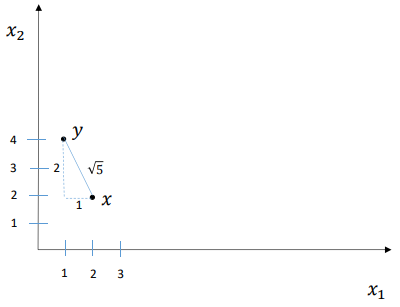
\includegraphics[width=5cm, height=3cm]{pic1}
  \end{itemize}
  \par
\vspace{6mm}
\subsubsection{Open Balls (neighborhoods)}
An open ball $B_{\varepsilon}(x) = \left\{ y \in \mathbb{R}_{+}^{n}: d(x,y) < \varepsilon \right\}$ is the set of points that are closer in Euclidean distance to $x \in \mathbb{R}_{+}^{n}$ than some real number $\varepsilon > 0$ \par \vspace{0.3em}
  \underline{Alternative Definition}: the open ball $B_{\varepsilon}(x)$ with radius $\varepsilon > 0$ and center $x \in \mathbb{R}^{m}$ is the set of points $y \in \mathbb{R}^{m}$ with distance less than $r$ from $x$, i.e. $B_{\varepsilon}(x) = \left\{ y \in \mathbb{R}^{m}: \ ||y - x|| < \varepsilon \right\}$
  \begin{itemize}
    \item  \underline{Note}: the theorem must contain $<$ instead of $\leq$ because otherwise the ball would contain its boundary points making it a closed instead of open ball. In otherwords, for an open ball each point in the element must be less than a selected radius on a plane
  \end{itemize}
  \par
  \underline{Example 1}: in $\mathbb{R}_{+}^{1}$ an open ball is an open interval on the number line. For $B_{1.5}(3)$ the circles at the endpoints of the interval $(1.5, 3.5)$ indicate that $1.5$ and $3.5$ are not in the open ball
  \begin{itemize}
    \item  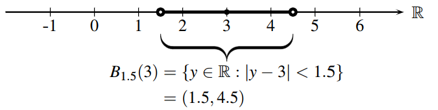
\includegraphics[width=5cm, height=3cm]{pic2}
  \end{itemize}
  \par
  \underline{Example 1}: for $x = (2,2)$ and $\varepsilon = 1$, the open ball $B_{\varepsilon}((2,2)) = \left\{ y \in \mathbb{R}^{n}_{+}: \ \sqrt{(y_{1} - 2)^{2} + (y_{2} - 2)^{2}} < 1 \right\}$
  \begin{itemize}
    \item  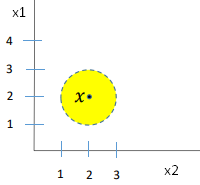
\includegraphics[width=5cm, height=3cm]{pic3}
  \end{itemize}
  \par
\vspace{6mm}
\subsubsection{Open Set}
A set $A \subseteq \mathbb{R}_{+}^{n}$ is open if and only if for each point $x \in A$ there is a radius $\varepsilon_{x} > 0$ such that the open ball $B_{\varepsilon}(x) \subseteq A$ \par \vspace{0.3em}
  \underline{Alternative Definition}: a set $S \in \mathbb{R}^{m}$ is open if and only if for each $x \in S$ there exists an open ball around $x$ that is completely contained in $S$ \par
  \underline{Boundary Points}: open sets cannot contain their boundary points, in other words the limit is not in the set since there is no open ball around $limit_{x}$ that is entirely in S. This distinguishes open sets from closed sets \par
  \underline{Theorem 1}: every open ball $A = B_{\varepsilon}(x)$ is an open set
  \begin{itemize}
    \item  \underline{Proof Outline}: take an arbitrary point $y$ in $B_{\varepsilon}(x)$ and prove that any arbitrary point $z$ contained in $B_{\varepsilon'}(y)$ is also contained in $B_{\varepsilon}(x)$
    \item  \underline{Proof}: take an arbitrary point $y$ in $B_{\varepsilon}(x)$. We need to show that there is an open ball $B_{\varepsilon'}(y)$ around $y$ that is contained in $B_{\varepsilon}(x)$. To do this, we prove that taking an arbitrary point $y$ in $B_{\varepsilon}(x)$ implies that $d(x,y) < \varepsilon$. Let $\varepsilon' = \varepsilon - d(x,y) > 0$, we have that $d(x,y) = \varepsilon - \varepsilon'$. Using $d(x,y) = \varepsilon - \varepsilon'$ and picking an arbitrary $z \in B_{\varepsilon'}(y)$ we can show that $d(x,z) < \varepsilon$. By triangular inequality, $d(x,z) \leq d(x,y) + d(y,z)$ and plugging $d(x,y) = \varepsilon - \varepsilon'$ into this yields $d(x,z) \leq \varepsilon - \varepsilon' + d(y,z)$. Since $z$ is contained in $B_{\varepsilon'}(y)$, it must be that $d(y,z) < \varepsilon'$. Using $d(y,z) < \varepsilon'$ yields $d(x,z) \leq \varepsilon - \varepsilon' + d(y,z) < \varepsilon - \varepsilon' + \varepsilon' = \varepsilon$. Since every point $z$ is contained in $B_{\varepsilon'}(y)$, $d(x,z) < \varepsilon$ implies that $d(x,y) < \varepsilon$. Therefore, $B_{\varepsilon'}(y) \subseteq B_{\varepsilon}(x)$.
    \item  \underline{Logic}: since $\varepsilon$ can be infinitismal, the infinitismal open ball $B_{\varepsilon}(y)$ contained in the open ball $B_{\varepsilon}(x)$ does not contain the boundary points of $B_{\varepsilon}(x)$
  \end{itemize}
  \par
  \underline{Theorem 2}: $A = \mathbb{R}^{n}$ is open in $\mathbb{R}^{n}$, $A = \mathbb{R}^{n}_{+}$ is open in $\mathbb{R}^{n}_{+}$
  \begin{itemize}
    \item  \underline{Logic 1}: take a point on the boundary. Since, by definition, open balls only include elements contained in $\mathbb{R}^{n}$ then any open ball that goes around the boundary point excludes points outside $\mathbb{R}^{n}$. The same is true for $R^{n}_{+}$ if we consider only positive natural numbers in our universe and therefore restrict the definition of open balls to only include points in $\mathbb{R}_{+}^{n}$. In otherwords, every point that is in the ball is in the universe
    \item  \underline{Logic 2}: take any point $x \in A$ and let $\varepsilon_{x} = \min \left\{x_{1}, x_{2}, \dots, x_{n} \right\}$. Then every point in the open ball $B_{varepsilon_{x}}(x) \in \mathbb{R}_{+}^{n}$. For example, let $x = (3,4) \in R_{+}^{2}$ and therefore $\varepsilon_{x} = \min \left\{ 3, 4 \right\} = 3$ - every point $y$ in the open yellow ball will be in $\mathbb{R}_{+}^{2}$ since each point $y$ satisfies $y_{i} > 0$ for $i = 1, 2$.
  \end{itemize}
  \par
  \underline{Theorem 3}: $A = \varnothing$ is open in $\mathbb{R}_{+}^{n}$
  \begin{itemize}
    \item  \underline{Proof}: observe that the conditions of openness of a set is satisfied if each $x \in A$ has an open neighbourhood in $A$. Since there is no $x$ in $A = \varnothing$, it follows that each $x \in A$ has an open ball in $A$
    \item  \underline{Both Open and Closed}: the empty set $\varnothing$ is both open and closed, this is as $\forall x \in \varnothing$ $x$ is an interior point (i.e. is open) and since the set of boundary points of $\varnothing$ is the empty set (i.e. is closed)
    \begin{itemize}
      \item  \underline{Complement}: since the complement of $A = \varnothing$ is $\mathbb{R}_{+}^{n}$ and the complement of $A = \mathbb{R}_{+}^{n}$ is $\varnothing$ then both $\mathbb{R}_{+}^{n}$ and $\varnothing$ are closed
    \end{itemize}
  \end{itemize}
  \par
\vspace{6mm}
\subsubsection{Closed Set}
A set $A \subset \mathbb{R}_{+}^{n}$ is closed if and only if the complement $A^{c} = \left\{ x \in \mathbb{R}_{+}^{n}: \ x \notin A \right\}$ of A is an open set \par \vspace{0.3em}
  \underline{Alternative Definition}: a set $S \in \mathbb{R}^{m}$ is closed if, whenever $\left\{ x_{n} \right\}_{n=1}^{\infty}$ is a convergent sequence completely contained in $S$, its limit is also contained in $S$ - in other words, a set $S \subseteq \mathbb{R}^{m}$ is closed if it contains all of its boundary points
  \par
  \underline{Example 1}: continuing from example 1 of open balls, the complement of the yellow open ball is a closed set. Formally, this is the entire positive quadrant excluding the yellow open ball, $A^{c} = \left\{ x \in \mathbb{R}_{+}^{n}: \ x \notin B_{1}((2,2)) \right\}$
  \begin{itemize}
    \item  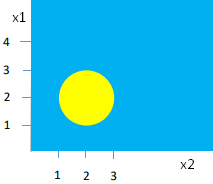
\includegraphics[width=5cm, height=3cm]{pic4}
  \end{itemize}
  \par
\vspace{6mm}
\subsubsection{DeMoran's Laws}
(Law 1) the complement of the union of any family of sets is equal to the intersection of the complements of the family \\ (Law 2) the complement of the intersection of any family of sets is equal to the union of the complements of the family \par \vspace{0.3em}
  \underline{Implications}: (1) the empty set $\varnothing$ and universal set $\mathbb{R}_{+}^{n}$ are both closed and open, (2) the union of any finite family of closed(open) sets is closed(open), (3) the intersection of any family of closed(open) sets is closed(open)
  \begin{itemize}
    \item  \underline{Finite Intersection Logic}: if we take the intersection of two finite open sets $A = \cap_{K \in \mathbb{N}} (1 - \tfrac{1}{k}, 1 + \tfrac{1}{k})$ then only $1 \in A$ and $A = \left\{ 1 \right\}$ is not open
    \item  \underline{Note}: implications 2 and 3 arise by combining Law 1 and Law 2
  \end{itemize}
  \par
\vspace{6mm}
\subsubsection{Bounded Set}
A set $A \subseteq \mathbb{R}_{+}^{n}$ is bounded if and only if we can put an open ball in $\mathbb{R}^{n}$ around the set $A$ \par \vspace{0.3em}
  \underline{Alternative Definition}: a set is bounded if there is an open ball that contains it, i.e. $S \subseteq R^{m}$ is bounded if $\exists K > 0: \ ||x|| < K, \ \forall x \in S$ \par
  \underline{Example}: the left image is bounded, the right is not bounded
  \begin{itemize}
    \item  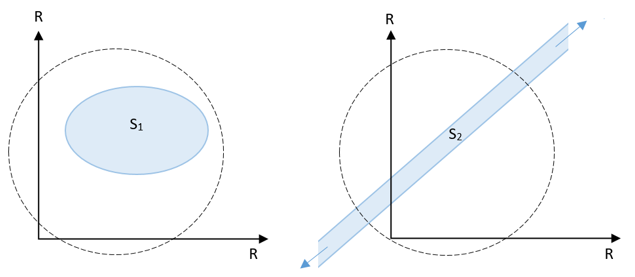
\includegraphics[width=5cm, height=3cm]{pic5}
  \end{itemize}
  \par
\vspace{6mm}
\subsubsection{Compact Set}
A set $A \subseteq \mathbb{R}_{+}^{n}$ is bounded if and only if it is both closed and bounded \par \vspace{0.3em}
  \underline{Example}: $B_{1} = \left\{ (x_{1},x_{2}) \in mathbb{R}^{2}: p_{1}x_{1} + p_{2}x_{2} \leq w \right\}$ is closed but not bounded. However, $B_{2} = \left\{ (x_{1},x_{2}) \in \mathbb{R}^{2}: p_{1}x_{1} + p_{2}x_{2} \leq w, x_{1} \geq 0, x_{2} \geq 0 \right\}$ is closed and bounded and therefore compact.
  \par
\vspace{6mm}
\subsubsection{Convex Set}
A set $A \subseteq \mathbb{R}_{+}^{n}$ is a convex set if and only if for all $x, y \in A$, and each $\alpha \in [0,1]$, the point $\alpha x + (1- \alpha)y$ is also in A \par \vspace{0.3em}
  \underline{Alternative Definition}: a set $S \subseteq \mathbb{R}^{n}$ is convex if and only if for every two points of the set the line segment between the two points also belongs to the set
  \par
  \underline{Example 1}: parts (a) and (b) are convex sets since all points between any two points are contained in the set, parts (c) and (d) are not convex sets since they contain two points where points between them are not contained in the set
  \begin{itemize}
    \item  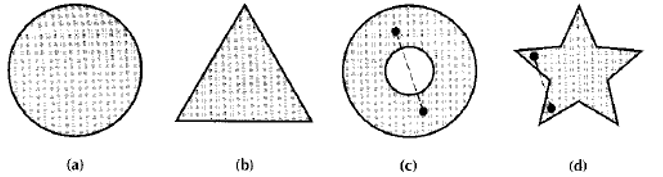
\includegraphics[width=5cm, height=3cm]{pic8}
  \end{itemize}
  \par
  \underline{Example 2}: suppose we have two bundles $x = (2,3)$ and $y = (4,7)$ for goods $x_{1}$ and $x_{2}$. Using $\alpha = \tfrac{1}{3}$, is the set $x, y \in A$ convex?
  \begin{itemize}
    \item  \underline{Answer}: $\alpha (2,3) + (1- \alpha)(4,7) = \tfrac{1}{3}(2,3) + \tfrac{2}{3}(4,7)$. This yields $(\tfrac{1}{3}(2) + \tfrac{2}{3}(4), \tfrac{1}{3}(3) + \tfrac{2}{3}(7)) = (\tfrac{10}{3}, \tfrac{17}{3}) = (x_{1}', x_{2}')$ which is contained in $A$ and therefore convex.
  \end{itemize}
  \par
  \underline{Example 3}: the below figure is convex though not closed
  \begin{itemize}
    \item  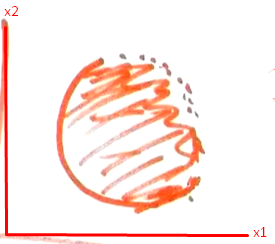
\includegraphics[width=4cm, height=3cm]{pic14}
  \end{itemize}
  \par
  \underline{Example 3}: the below budget sets are not convex
  \begin{itemize}
    \item  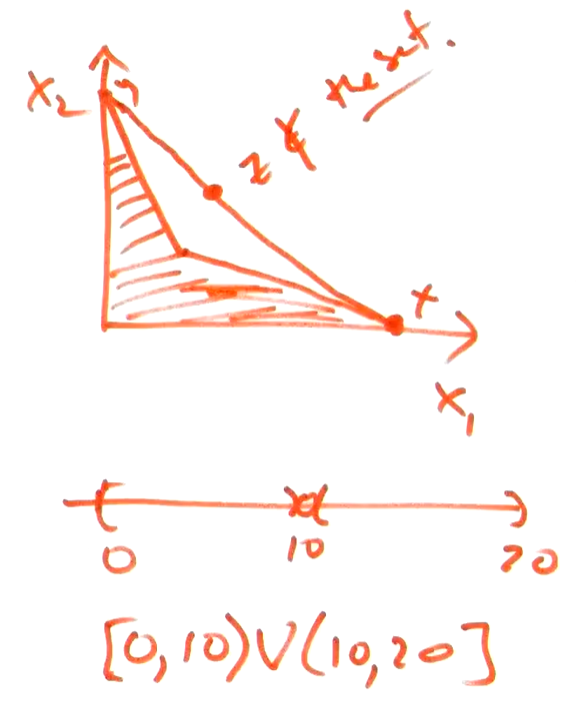
\includegraphics[width=4cm, height=7cm]{pic15}
  \end{itemize}
  \par
\vspace{6mm}
\subsubsection{Convergent Sequences}
Occurs when for all $\varepsilon > 0$ there exists a $\mathbb{N}$ such that for all values of $n$ greater than $\mathbb{N}$ the $n^{th}$ \textit{elements value in the sequence minus the limit's value} will be less than $\varepsilon$ \par \vspace{0.3em}
  \underline{Mathemtical Definition}: let $(x_{n})_{n \in \mathbb{N}}$ be a sequence with codomain $\mathbb{R}$. We say that $(x_{n})$ converges to $x^{*}$ or that $x^{*}$ is the limit of $(x_{n})_{n \in \mathbb{N}}$ if: $\forall \varepsilon > 0 \exists N \in \mathbb{N} \forall n \geq N: \ |x_{n} - x^{*}| < \varepsilon$ \par
  \underline{Sequence}: a sequence of real numbers is an assignment of a real number to each natural number. In other words, $f: N \rightarrow X$ is a function that matches a set of natural numbers, $n$, to a set of numbers, $x$. A sequence with a limit is called convergent
  \begin{itemize}
    \item  \underline{Convergence Defined by the Limit of a Sequence}: let $\left\{ x_{1}, x_{2}, x_{3} \right\}$  be a sequence of real numbers and let $r$ be a real number. We say that $r$ is the limit of this sequence if for any small positive number $\varepsilon$, there is a positive integer $N$ such that for all $n \geq N: \ |x_{n} - r| < \varepsilon$, i.e. $x_{n}$ is in the interval about $r$ given $\varepsilon$ for all $n$ past given point $N$
  \end{itemize}
  \par
\vspace{6mm}
\subsubsection{Continuous Functions}
A function $f: \mathbb{R}_{+}^{n} \rightarrow \mathbb{R}$ is continuous if and only if the inverse image $f^{-1} (B) = \left\{ x \in \mathbb{R}_{+}^{n}: f(x) \in B \right\}$ of each open ball $B$ in the range $\mathbb{R}$ is also open in the doman $\mathbb{R}_{+}^{n}$ \par \vspace{0.3em}
  \underline{Alternative Definition 1}: let $D \subseteq \mathbb{R}^{k}$. A function $f: D \rightarrow \mathbb{R}^{m}$ is continuous at $x = (x_{1}, x_{2}, \dots, x_{k}) \in D$ if for every sequence $(x_{n})_{n \in \mathbb{N}} \in D$ that converges to x, the sequence $(f(x_{n}))_{n\in \mathbb{N}} \in \mathbb{R}$ converges to $f(x)$. The function is continuous if it is continuous at $x$ for all $x \in D$ \par
  \underline{Explanation}: a function that maps nearby points into nearby points - i.e. you can draw the graph of the function without lifting your pencil from the paper. In other words, if we want to get all the $f(x)$ values to stay in some small neighborhood around $f(x_{0})$ we simply need to choose a small enough neighborhood for the $x$ values around $x_{0}$. If we can do that no matter how small the $f(x)$ neighborhood is, then $f$ is continuous at $x_{0}$ \par
  \underline{Continuous Example}: the below function is continuous as for any $x_{0}$ that we select and converges, the codomain converges to $y_{0}$
  \begin{itemize}
    \item  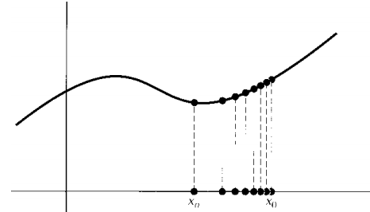
\includegraphics[width=5cm, height=3cm]{pic6}
  \end{itemize}
  \par
  \underline{Discontinuous Example}: the function $f(x) = \left\{ 1 \ \text{if} \ x > 0, 0 \ \text{if} \ x \leq 0 \right\}$ is not continuous as the codomain does not converge to the $y_{0}$ given by the $x_{0}$ selected. In other words, for $\varepsilon < 1$ the definition of convergence is violated at $x_{0} = 0$
  \begin{itemize}
    \item  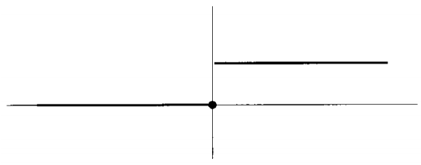
\includegraphics[width=5cm, height=3cm]{pic7}
  \end{itemize}
  \par
  \underline{Using original definition}: the image of $f(x)$ consists of all the elements of $y$ that an element of $x$ is mapped to. If $f(x) = \left\{x \ \text{if} \ x < 10, x + 10 \ \text{if} \ x \geq 10 \right\}$ and we set the inverse image open ball $B = (15, 25)$, then  we have that $f^{-1}(15,25) = \left\{ x \in \mathbb{R}: \ f(x) \in (15, 25) \right\} = [10, 15)$. This is as $x \geq 10$ is not open in the domain for the open ball in the range $f^{-1}(15,25)$
  \par
\vspace{6mm}
\subsubsection{Concave Functions}
$f$ is concave if and only if $\forall x,y$ and all $t \in [0,1]$ we have that $f(\alpha x + (1-\alpha)y) \geq \alpha f(x) + (1-\alpha)f(y) $\par \vspace{0.3em}
\subsubsection{Homogeneous of Degree k}
A real value function $f$ defined on a subset $X$ of $\mathbb{R}^{n}$ is \textit{homogeneous of degree k} if and only if $f(tx) = t^{k}f(x)$ for all $t \in \mathbb{R}_{++}$ and all $x \in X$ \par \vspace{0.3em}
  \underline{Properties}: if you mutliply all inputs by a constant ($t > 0$) then you will generate an output equal to $t^{k}$ times the function, for instance if $k=1$ and you multiply all inputs by $t=2$ then you will get twice the output while if $k = 2$ you will get four times the output
  \par
  \underline{Degree Zero}: if a function is homogeneous of degree zero, this means that multiplying all variables in its domain (inputs) by $t > 0$ will cause no change in its co--domain (outputs). In other words, for a demand function we have that $t^{0}x(p, I) = x(tp, tI) = x(p,m)$
  \par
  \underline{Budget Exhaustion Theorem}: if the consumer demand function $x_{i}(p,I), \ i = 1, \dots, n$ is homogenuous of degree zero in all prices and income then it satisfies budget exhaustion where $p \cdot x(p,y) = I, \ \forall (p,I)$
  \begin{itemize}
    \item  \underline{Logic}: if you are doubling income and doubling prices and it means you are suddenly consuming more than double of a given good it must mean that before you were not spending all your income on that good (assuming we are in a one good world)
  \end{itemize}

\newpage

\section{Consumer Theory}

\vspace{2.5mm}
\subsection{Preferences}
In this section the concepts of preference relations will be explored. In addition to this, the consumer choice axioms will be outlined to provide a framework for proving and understanding utility representations \par
\vspace{6mm}
\subsubsection{Preference Relation}
Preferences are defined for each consumer over bundles of goods, with the notation $\succeq$ meaning \textit{at least as good as} \par \vspace{0.3em}
  \underline{Preferences Definition}: preferences of a consumer on the set of bundles in $\mathbb{R}_{+}^{n}$ is a subset $\succeq$ of $\mathbb{R}_{+}^{n} \times \mathbb{R}_{+}^{n}$. In mathematics, this subset is referred to as a \textit{binary relation} on the set $\mathbb{R}_{+}^{n}$
  \begin{itemize}
    \item  \underline{Note}: $\mathbb{R}_{+}^{n}$ is the set of all bundles in the universe, while $\mathbb{R}_{+}^{n} \times \mathbb{R}_{+}^{n}$ is the set of all pairs of bundles in the universe. For instance, if we $A = \left\{a, b, c\right\}$ then  $A \times A = \left\{(a,a), (a,b), (a,c), (b,a), (b,b), (b,c), (c,a), (c,b), (c,c) \right\}$
  \end{itemize}
  \par
  \underline{Examples}
  \begin{itemize}
    \item  \underline{Example 1}: $\succeq = \mathbb{R}_{+}^{n} \times \mathbb{R}_{+}^{n}$ represents the case where every possible bundle is at least as good as every other
    \item  \underline{Example 2}: $\succeq = \varnothing$ represents the case where no bundle is at least as good as any other (including itself
    \item  \underline{Example 3}: $\succeq = \left\{ (x,y) \in \mathbb{R}_{+}^{n} \times \mathbb{R}_{+}^{n}: \ x_{i} \geq y_{i} \ \text{for all} \ i = 1, \dots, n \right\}$ represents the case where only bundles where one has at least as much of each good as the other can be compared
    \item  \underline{Example 4}: $\succeq = \left\{ (x,y) \in \mathbb{R}_{+}^{n} \times \mathbb{R}_{+}^{n}: \ \prod_{i=1}^{n} x_{i} \geq \prod_{i=1}^{n} y_{i} \right\}$ represents the case where all bundles are compared and on is at least as good as another whenever the product of quantities is higher. See below for a graphical representation where $x_{1}x_{2} = 2$, red represents the better than sets and blue the worse than sets
    \begin{itemize}
      \item  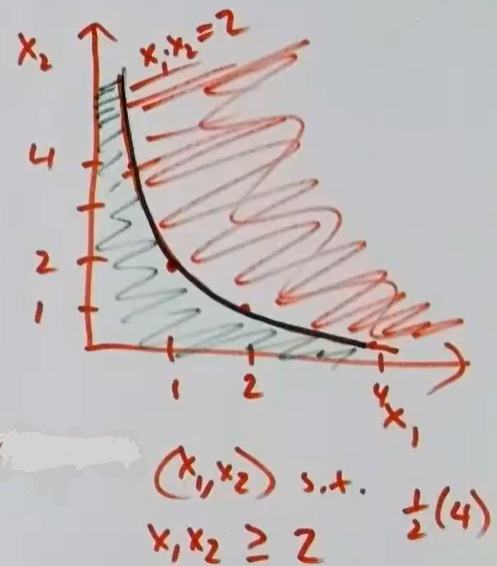
\includegraphics[width=4cm, height=3cm]{pic12}
    \end{itemize}
  \end{itemize}
  \par
\vspace{6mm}
\subsubsection{Strict and Indifferent Preference Relations}
To define instances where a consumer is indifferent between a set of bundles or strictly prefers a given bundle over another, we use indifferent and strict preference relations \par \vspace{0.3em}
  \underline{Strict Preference Relation}: when the binary relation $\succ$ on the consumption set $X$ is defined as follows; $x_{1} \succ x_{2}$ if and only if $x_{2} \nsucceq x_{1}$. This is read $x_{1}$ is strictly preferred to $x_{2}$
  \begin{itemize}
    \item  \underline{Implication 1}: from $\succeq = \mathbb{R}_{+}^{n} \times \mathbb{R}_{+}^{n}$ we have that $\succ = \varnothing$ and therefore there is no strict preference
    \item  \underline{Implication 2}: from $\succeq = \varnothing$ we have that $\succeq = \varnothing$ and therefore none are strict
    \item  \underline{Implication 3}: from $\succeq = \left\{ (x,y) \in \mathbb{R}_{+}^{n} \times \mathbb{R}_{+}^{n}: \ x_{i} \geq y_{i} \ \text{for all} \ i = 1, \dots, n \right\}$ we get that $$\succ = \left\{ (x,y) \in \mathbb{R}_{+}^{n} \times \mathbb{R}_{+}^{n}: \ x_{i} \geq y_{i} \ \text{for all} \ i = 1, \dots, n \ \text{and} \ x_{i}>y_{j} \ \text{for some} \ j = 1, \dots, n \right\}$$Therefore, a bundle is strictly preferred to $y$ if and only if $x$ has  at least as much of each commodity as y and stricty more of some commodity
    \item  \underline{Implication 4}: from $\succeq = \left\{ (x,y) \in \mathbb{R}_{+}^{n} \times \mathbb{R}_{+}^{n}: \ \prod_{i=1}^{n} x_{i} \geq \prod_{i=1}^{n} y_{i} \right\}$ we get that $$\succ = \left\{ (x,y) \in \mathbb{R}_{+}^{n} \times \mathbb{R}_{+}^{n}: \ \prod_{i=1}^{n} x_{i} > \prod_{i=1}^{n} y_{i} \right\}$$Therefore, we have strict preference only when the product is higher
  \end{itemize}
  \par
  \underline{Indifference Reation}: when the binary relation $\sim$ on the consumption set $X$ is defined as follows; $x_{1} \sim x_{2}$ if and only if $x_{1} \succeq x_{2}$ a nd $x_{2} \succeq x_{1}$. is is read as $x_{1}$ is indifference to $x_{2}$
  \begin{itemize}
    \item  \underline{Implication 1}: from $\succeq = \mathbb{R}_{+}^{n} \times \mathbb{R}_{+}^{n}$ we have that $\sim = \mathbb{R}_{+}^{n} \times \mathbb{R}_{+}^{n}$ and therefore all bundles are indifferent
    \item  \underline{Implication 2}: from $\succeq = \varnothing$ we get $\sim = \varnothing$
    \item  \underline{Implication 3}: from $\succeq = \left\{ (x,y) \in \mathbb{R}_{+}^{n} \times \mathbb{R}_{+}^{n}: \ x_{i} \geq y_{i} \ \text{for all} \ i = 1, \dots, n \right\}$ we get that $$\sim= \left\{ (x,y) \in \mathbb{R}_{+}^{n} \times \mathbb{R}_{+}^{n}: \ x = y \right\}$$Therefore, each bundle is indifferent only to itself
    \item  \underline{Implication 4}: from $\succeq = \left\{ (x,y) \in \mathbb{R}_{+}^{n} \times \mathbb{R}_{+}^{n}: \ \prod_{i=1}^{n} x_{i} \geq \prod_{i=1}^{n} y_{i} \right\}$ we get that $$\sim = \left\{ (x,y) \in \mathbb{R}_{+}^{n} \times \mathbb{R}_{+}^{n}: \ \prod_{i=1}^{n} x_{i} = \prod_{i=1}^{n} y_{i} \right\}$$ Therefore, indifference when the product of the quantities is the same
  \end{itemize}
  \par
  \underline{Combining Implications of Indifference and Strict Preference}: from implications 2 we have that both indifference and strict preferences require that "one is atleast as good as the other". The combination of the strict preference implication $i$ and indifference implication $i$ yields example $i$ from the preference relation section \par
\vspace{6mm}
\subsubsection{Lexicographic Preferences}
Describe preferences where an agent prefers any amount of one good (X) to any amount of another (Y), therefore if offered several bundles then the agent will choose the bundle that offers the most $X$ no matter how much $Y$ there is \par \vspace{0.3em}
  \underline{Idea}: first compare two bundles $x$ and $y$ according to the quantity of the the first good. If one bundle has more than the other of that good, then the one having more is strictly preferred. If neither has more of that good, go to the next good and compare in the same way. Repeat this until one bundle has more of good $z$ than the other bundle, where $z$ is the most recently compared good (i.e. the good with the lowest rank of those compared so far). If there is no bundle with more of good $z$, then the bundles are deemed to be indifferent to each other as they are the same bundle \par
  \underline{Example for Two Goods}: $\mathbb{R}_{+}^{2}: \ x \succeq y$ if and only if (a) $x_{1} > y_{1}$ or (b) $x_{1} = y_{1}$ and $x_{2} \geq y_{2}$
  \begin{itemize}
    \item  \underline{Cases}: for $(1,2)$ vs $(2,1)$ the latter has more of the first good so is strictly preferred, for $(1,2)$ vs $(1,1)$ both have same amounts of the first good but the former has more of the second good so it is preferred, for $(1,2)$ and $(1,2)$ both have the same amount of the first and second goods so they are indifferent. This is shown in the below figure where bundle $x = (x_{1}, x_{2}) = (2,1)$ and what is marked in red are the $y \succeq x$ bundles that follow $\succeq$, note that the dotted red line is open to represent the boundary point where the $y \succeq x$ relationship does not hold
    \begin{itemize}
      \item  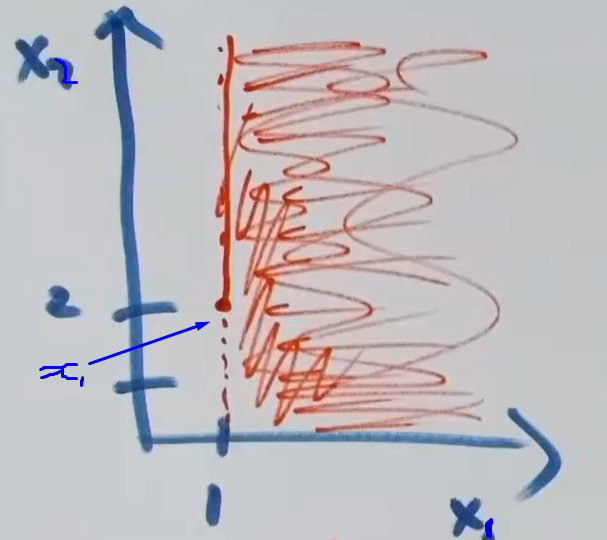
\includegraphics[width=4cm, height=3cm]{pic11}
    \end{itemize}
    \item  \underline{Defining by Strict and Indifference Preferences}: from $\succeq$ we have that:
    \begin{itemize}
      \item  \underline{A}: $\sim = \left\{(x,y) \in \mathbb{R}_{+}^{n} \times \mathbb{R}_{+}^{n}: \ x = y \right\}$ so each bundle is indifferent only to itself
      \item  \underline{B}: $\succ = \left\{(x,y) \in \mathbb{R}_{+}^{n} \times \mathbb{R}_{+}^{n}: \ x_{1} > y_{1} \ \text{or} \ (x_{1} = y_{1} \ \text{and} \ x_{2} > y_{2}) \right\}$ so a bundle is strictly preferred to another if and only if it has more of the first good or equal amounts of the first and more of the second.
    \end{itemize}
  \end{itemize}
  \par
\vspace{6mm}
\subsubsection{Convex Preferences}
Preferences $\succeq$ are convex if and only if for each $x \in \mathbb{R}_{+}^{n}$ the least as good as set $G(x)$ is a convex set \par \vspace{0.3em}
  \underline{Alternative Definition}: preferences are convex if and if for all $x, y \in \mathbb{R}_{n}^{+}$ and all $t \in [0,1]$: if $x \succeq y$ then $tx + (1-t)y \succeq y$
  \begin{itemize}
    \item  \underline{Interpretation}: averages are at least as good as extremes, i.e. you will have convex or straight shaped indifference curves
  \end{itemize}
  \par
  \underline{Strictly Convex Preferences}: preferences $\succeq$ are strictly convex if and only if all distinct $x,y \in \mathbb{R}_{+}^{n}$ and all $t \in (0,1)$, if $x \succeq y$ then $tx + (1-t)y \succ y$
  \begin{itemize}
    \item  \underline{Interpretation}: avarages are better than extremenes, i.e. you will only have convex shaped indifference curves
  \end{itemize}
  \par
  \underline{Utility Representation}: the utility representation of convex preferences is quasi-concavity
  \par
  \underline{Example 1}: the below figure has convex preferences
  \begin{itemize}
    \item  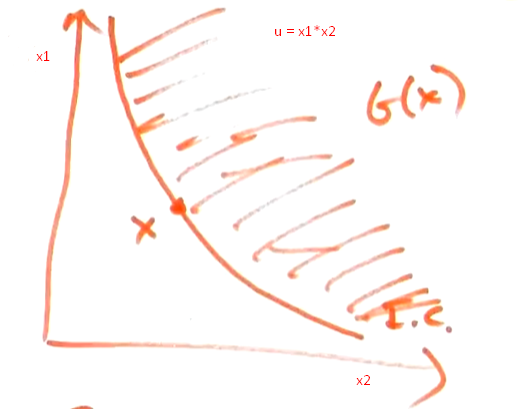
\includegraphics[width=4cm, height=3cm]{pic16}
  \end{itemize}
  \par
  \underline{Example 2}: the below figure, though is not closed, has convex preferences
  \begin{itemize}
    \item  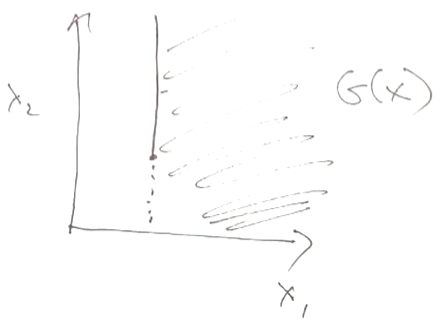
\includegraphics[width=8cm, height=6cm]{pic17}
  \end{itemize}
  \par
\vspace{6mm}
\subsubsection{Consumer Choice Axioms}
All bundles in the subset can be compared (completeness), choices are consistent (transitivity), the consumer can choose all bundles in the subset (continuity), and more is always better (strict monotonicity). These four axioms must hold for preferences to be considered 'rational' \par \vspace{0.3em}
  \underline{Axiom 1 - Completeness}: for all $x_{1}$ and $x_{2}$ in $X$, either $x_{1} \succeq x_{2}$ or $x_{2} \succeq x_{1}$ \par
  \underline{Axion 2 - Transitivity}: for any three elements $x_{1}, x_{2}, x_{3}$ in $X$, if $x_{1} \succeq x_{2}$ and $x_{2} \succeq x_{3}$ then $x_{1} \succeq x_{3}$
  \begin{itemize}
    \item  \underline{Note}: although we require only that the consumer be capable of comparing two alternatives at a time, the assumption of transitivity requires that otther pairwise comparisons be linked together in a consistent way
    \item  \underline{Transitivity Transfers to Indifference and Strict}: suppose that preferences $\succeq$ are transitive, then:
    \begin{itemize}
      \item  \underline{1}: indifference and strict preferences are transitive
      \item  \underline{2}: for all $x, y, z \in \mathbb{R}_{+}^{n} \times \mathbb{R}_{+}^{n}$ if $x \succeq y$ and $y \succeq z$ (with one indifference), then $x \succeq z$
      \item  \underline{3}: for all $x, y, z \in \mathbb{R}_{+}^{n} \times \mathbb{R}_{+}^{n}$ if $x \succeq y$ and $y \succeq z$ (with at least one strict), then $x \succ y$
    \end{itemize}
  \end{itemize}
  \underline{Theorem 1}: preferences $\succeq$ are complete and transitive if and only if preferences $\succ$ are negative transitive and asymmetric
  \begin{itemize}
    \item  \underline{Negative Transitivity}: occurs when $x \nsucc y$ and $y \succ z$ implies that $x \nsucc z$
    \item  \underline{Asymmetic}: $x \succ y$ implies that $y \nsucc x$
  \end{itemize}
  \par
  \underline{Axiom 3 - Continuity}: for all $x \in \mathbb{R}_{+}^{n}$, the "at least as good as set" $\succeq (x)$ and the "no better than" set $\preceq (x)$ are closed in $\mathbb{R}_{+}^{n}$
  \begin{itemize}
    \item  \underline{Conditions from Definition} preferences are continuious if $G(x) = \left\{ y \in \mathbb{R}_{+}^{n}: \ y \succeq x \right\}$ and $W(x) = \left\{ y \in \mathbb{R}_{+}^{n}: \ x \succeq y \right\}$ are both closed in $\mathbb{R}_{+}^{n}$
    \item  \underline{Theorem 1}: suppose that preferences are complete. Then, they are continuous if and only if for all $x \in \mathbb{R}_{+}^{n}$ the sets $SG(x) = \left\{ y \in \mathbb{R}_{+}^{n}: \ y \succ x \right\}$ and $SW(x) = \left\{ y \in \mathbb{R}_{+}^{n}: \ x \succ y \right\}$ are open in $\mathbb{R}_{+}^{2}$
    \begin{itemize}
      \item  \underline{Logic}: $SG(x)$ follows by definition of continuity and completeness when taking the complement of $W(x)$, $SW(x)$ follows by definition of continuity and completeness when taking the complement of $G(x)$
      \item  \underline{Note}: $SG(x)$ is referred to as the strictly greater than $x$ set while $SW(x)$ is referred to as the strictly worse than $x$ set
    \end{itemize}
  \end{itemize}
  \par
  \underline{Axiom 4 - Strict Monotonicity}: for all $x_{0}, x_{1} \in \mathbb{R}_{+}^{n}$, if $x_{0} \geq x_{1}$ then $x_{0} \succeq x_{1}$ while if $x_{0} > x_{1}$ then $x_{0} \succ x_{1}$
  \begin{itemize}
    \item  \underline{Alternative Definition}: if $x$ has at least as much of each good as $y$ and strictly more of some good, then $x \succ y$
    \begin{itemize}
      \item  \underline{Note}: by completeness of preferences, the alternative definition implies the first definition
    \end{itemize}
    \item  \underline{Exercise 1}: prove that the alternative definition implies the first definition given the requirement that preferences are complete
    \begin{itemize}
      \item  \underline{Answer}: the first part of the definition states that if $x \geq y$ then $x \succeq y$, which gives us case (a) where $x = y$ and case (b) where $x \neq y$. For (a) we have that by completeness $x \succeq y$, for (b) x has atleast more of some good which by completness implies that $x \succ y$. Thus the two cases, (a) and (b), given by the first part of the definition imply the alternative definition. The second part of the definition states that if $x > y$ then $x \succ y$, by completeness this implies that \textit{x has atleast as much of good as y and strictly more of some good} which demonstrates equivalency to the alternative definition. Without completeness, these implications would not hold because it could mean that comparisons can only be made in the case where $x$ has \textit{strictly more of some good} and not \textit{strictly more of all goods}.
    \end{itemize}
  \end{itemize}
  \par
\vspace{6mm}
\subsubsection{Intermediate Value Version of Continuity}
If the preferences are continuous and complete, then for any $x, y, z \in \mathbb{R}_{+}^{n}$, if $x \succ y$ and $y \succ z$, then there is some $\alpha \in (0,1)$ such that the convex combination $\alpha x + (1- \alpha)z$ is indifferent to y. This resembles the \textit{intermediate value theorem} \par \vspace{0.3em}
  \underline{Proof}: this can be proved using completeness and continuity together with the least upper bound property (i.e. that every non-empty set of reals that is bounded above, has a least upper bound). We know that $x \succ y$ and $y \succ z$ and that the preferences are continuous. We need to show that there is some point on the line between $x$ and $z$ that is indifferent to $y$. Consider the set $A = \left\{ \alpha \in [0,1]: \ y \succ \alpha x + (1- \alpha)z \right\}$. It stands that $\alpha = 0$ is an element of $A$ since $0x + (1 - 0)z = z$ and $y \succ z$, therefore $A$ is a set of reals. It also stands that $\alpha = 1$ is not an element of $A$ since $1x + (1-1)z = x$ and $x \succ y$ meaning that, at $\alpha = 1,$ $\alpha x + (1- \alpha)z$ is not indifferent to $y$, therefore $A$ is bounded above by $1$ and must have a least upper bound equal to or less than $1$. Call the least upper bound $\alpha^{*}$, we can show that $\alpha^{*}x + (1 - \alpha_{*})z \sim y$ using the following steps:
  \begin{itemize}
    \item  \underline{Step 1}: show that $0 < \alpha^{*} < 1$ using completness and continuity around $x$ and around $z$. \\ For $0 < \alpha^{*}$ we have that by continuity theorem 1, since $y \succ z$, there is an open ball $B_{\varepsilon}(z)$ around $z$ such that every $z'$ in that ball that can be compared to $y$ satisfies $y \succ z'$. By completeness, all the stuff in the ball can be compared to $y$, in particular the stuff that is also on the line between $x$ and $z$. Note that if we have $\alpha < 0$ then there would be $z'$s in the open ball around $B_{\varepsilon}(z)$ that do not satisfy and contradict $y \succ z'$. Therefore, it must be that $0 < \alpha^{*}$. \\ For $\alpha_{*} < 1$ we have that by continuity theorem 1, since $x \succ y$, there is an open ball $B_{\varepsilon}(y)$ around $y$ such that every $y'$ in that ball that can be compared to $x$ satisfies $x \succ y$. Likewise, by completeness, it must be that $\alpha^{*} < 1$.
    \item  \underline{Step 2}: show that $\alpha^{*}x + (1 - \alpha_{*})z \sim y$ using completeness and continuity. By completeness either (1) $\alpha^{*}x + (1-\alpha^{*})z \succ y$, (2) $y \succ \alpha^{*}x + (1-\alpha^{*})z$, or (3) $\alpha^{*}x + (1-\alpha^{*})z \sim y$. \\ Option 1 cannot be the case as for $\alpha^{*}x + (1-\alpha^{*})z \succ y$ to hold we cannot have $\alpha^{*}$ as our upper bound \\ Option 2 cannot be the case since the least upper bound $1 \in \alpha^{*}$ the relationship $y \succ \alpha^{*}x + (1-\alpha^{*})z$ does not hold and so $\alpha^{*}$ is not an upper bound since an open ball around the point of our least upper bound would include points where $$y \nsucc \alpha^{*}x + (1-\alpha^{*})z$$ \\ Therefore, we are left with option (3), $\alpha^{*}x + (1-\alpha^{*})z \sim y$.
  \end{itemize}
  \par
  \underline{Usefulness}: this means that something on the line connecting $x$ and $z$ is indifferent to $y$
  \begin{itemize}
    \item  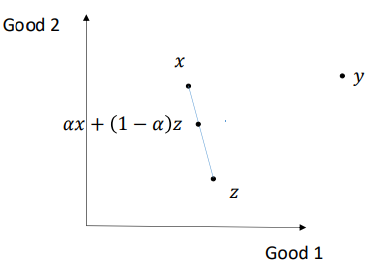
\includegraphics[width=6cm, height=4.5cm]{pic9}
  \end{itemize}
  \par
\vspace{6mm}
\subsubsection{Utility Representation}
A utility representation of preferences $\succeq$ is a real valued function $u: \mathbb{R}_{+}^{n} \rightarrow \mathbb{R}$ over the set of bundless such that for all bundles $x,y \in R_{+}$: \\ (a) if $x \succeq y$ then $u(x) \geq u(y)$ \\ (b) if $u(x) \geq u(y)$ then $x \succeq y$ \par \vspace{0.3em}
  \underline{Alternative Definition}: a real values function $u: \mathbb{R}_{+}^{n} \rightarrow \mathbb{R}$ is called a utility function representing the relation $\succeq$ if for all $x_{0}, x_{1} \in \mathbb{R}_{+}^{n}, u(x_{0}) \geq u(x_{1}) \Longleftrightarrow x_{0} \succeq x_{1}$ \par
  \underline{Strict Preferences}: $u: \mathbb{R}_{+}^{n} \rightarrow \mathbb{R}$ is a utility representation of preferences $\succeq$ if and only if for all bundles $x, y \in \mathbb{R}_{+}^{n}$: (a) if $x \succ y$ then $u(x) > u(y)$, (b) if $u(x) > u(y)$ then $x \succ y$ \par
  \underline{Theorem 1 - Existence of a Utility Representation}: if the binary relation $\succeq$ is complete, transitive, continuous, and strictly monotonic, then there exists a continuous real valued function, $u: \mathbb{R}_{+}^{n} \rightarrow \mathbb{R}$, which represents $\succeq$
  \begin{itemize}
    \item  \underline{Proof in Terms of 2 Goods}: \textbf{step 1} - show every point $x$ is indifferent to a point $y$ on the $45^{\circ}$ line which represents bundles with the same amount of each good, \textbf{step 2} - assign a utility $u(x)$ equal to the quantity of each good at the point on the diagonal that is indifferent to $x$, \textbf{step 3} - show that that if $x \succeq y$ then $u(x) \geq u(y)$, \textbf{step 4} - show that if $u(x) \geq u(y)$ then $x \succeq y$
    \begin{itemize}
      \item  \underline{Step 1}: if $x$ is on the $45^{\circ}$ line, we are done as by completeness $x \sim x$. Consider $x$ not on the $45^{\circ}$ line, let $\widetilde{x}$ be the bundle on the $45^{\circ}$ line where the amount of each good is the larger of $x_{1}$ and $x_{2}$ (e.g. if $x = (5,2)$ then $\widetilde{x} = (5,5)$). Since $\widetilde{x}$ has more of at least one good and at least as much of each of the others then $\widetilde{x} \succ x$ by strict monotonicity. Also, by strict monotinicity $\widetilde{x} \succ z$, where $z$ is the origin $(0,0)$. Hence, there is a point on the diagonal that is indifferent to $x$ by the \textit{intermediate value version of continuity} (i.e. $\exists \alpha, x = \alpha \widetilde{x} + (1-\alpha)z$). Note that, by strict monotonicity, there is only one bundle on the diagonal that is indifferent to $x$ referred to as $x^{d}$ where $x^{d} \sim x$
      \begin{itemize}
        \item  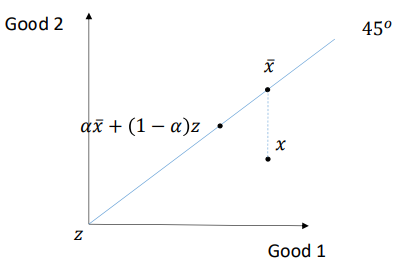
\includegraphics[width=4cm, height=3cm]{pic10}
      \end{itemize}
      \item  \underline{Step 2}: take the example where $x = (5,2)$ and the point on the diagonal that is indifferent to $x$ is $x^{d} = (2.5, 2.5)$ which yields $u(x) = 2.5$. Clearly, $u(x^{d}) = u(x)$ since $x^{d} = x$ in this case
      \item  \underline{Step 3}: suppose $x \succeq y$ and that by definition $x^{d} \sim x, y \sim y^{d}$. Therefore by transitivity we have that $x^{d} \succeq y^{d}$ and by strict monotonicity we can infer that $u(x^{d}) \geq u(y^{d})$.
      \begin{itemize}
        \item  \underline{Logic}: since $x^{d}$ and $y^{d}$ are both on the diagonal whereby $x^{d} = (a, a)$ and $y^{d} = (b,b)$ for some quantities $a$ and $b$. By strict monotonicity, combined with $x^{d} \succeq y^{d}$, we can infer that $a \geq b$. This is as, if on the contrary $b > a$, then $y^{d}$ would have more of each good than $x^{d}$. This would imply, by strict monotonicity, that $y^{d} \succ  x^{d}$. Since this would contradict the finding that $x^{d} \succeq y^{d}$, then it must be that $a \geq b$. Since $a$ represents the quantity of each good in $x^{d}$ and $b$ represents the quantity of each good in $y^{d}$, the utility function defined in step 2 will assign $u(x^{d}) = a$ and $u(y^{d}) = b$. Since $a \geq b$, we conclude that $u(x^{d}) \geq u(y^{d})$.
      \end{itemize}
      From $u(x^{d}) \geq u(y^{d})$ and $x^{d} \sim x, y \sim y^{d}$ we can infer that $u(x) \geq u(y)$. This is as by applying our utility function from step 2 we get $u(x) = u(x^{d}) \geq u(y^{d}) = u(y)$ and therefore $u(x) \geq u(y)$
      \item  \underline{Step 4}: \begingroup\color{blue} homework from priscilla notes \endgroup
    \end{itemize}
  \end{itemize}
  \par
  \underline{Finite Sets}: if the set of alternatives is finite or countably infinite, then we get a utility representation with only complete and transitive preferences \par
  \underline{Huge Spaces}: for the huge space $\mathbb{R}^{n}_{+}$, we can get a utility representation without monotonicity \par
  \underline{Properties}: (1) preferences represented by a utility function will always be complete and transitive, (2) preferences represented by a continuous utility function will always be continuous
  \begin{itemize}
    \item  \underline{Proof for (2)}: for $x \in \mathbb{R}^{n}_{+}$ we want to show $SG(x)$ is open. Suppose we have $x: \ (u(x), + \infty)$ which is open in $\mathbb{R}^{n}_{+}$. The inverse image of $x$ we have that $u^{-1}(u(x), + \infty) = \left\{y \in \mathbb{R}_{+}^{n}: u(y) \geq u(x) \right\} = SG(x)$ which by continuity is open. Therefore, since the inverse image is open, we have that the preferences represented by the continuous utility function are continuous.
  \end{itemize}
  \par
\vspace{6mm}
\subsubsection{Exercise 1}
Answer if the below preferences are are complete, transitive, continuous, and strongly monotonic? \par \vspace{0.3em}
  \begin{itemize}
    \item  \underline{Question 1}: $x \succeq y$ if and only if $(x_{1})^{2} + x_{2} \geq (y_{1})^{2} + y_{2}$
    \begin{itemize}
      \item  \underline{Complete}: take $x,y$, we have that either $x_{1}^{2} + x_{2} \geq y_{1}^{2} + y_{2}$ or $y_{1}^{2} + y_{2} > x_{1}^{2} + x_{2}$. Therefore, it is complete.
      \item  \underline{Transitive}: take $x,y,z$. Suppose $x \succeq y$ and $y \succeq z$. From the $\Rightarrow$ implication we have that $x_{1}^{2} + x_{2} \geq y_{1}^{2} + y_{2}$ and $y_{1}^{2} + y_{2} \geq z_{1}^{2} + z_{2}$, therefore $x_{1}^{2} + x_{2} \geq z_{1}^{2} + z_{2}$. From the $\Leftarrow$ implication we have that $x \succeq z$
      \item  \underline{Continuous}: since the preferences have a utility representation they must be continuous. Also, by drawing the indifference curves, it is clear that $G(x)$ and $W(x)$ is closed. Note that the complements $G(x) \rightarrow SG(x)$ and $W(x) \rightarrow SW(x)$ are open which implies that the preferences are continuous. \\
      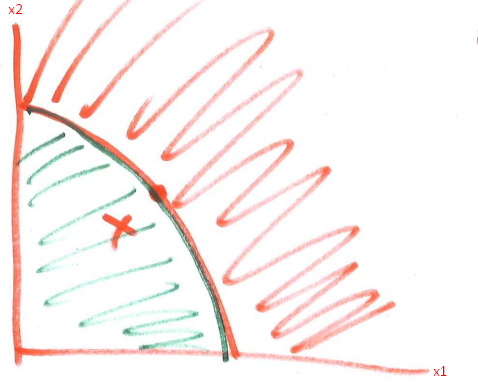
\includegraphics[width=4cm, height=3cm]{pic20}
      \item  \underline{Strongly Monotonic}: suppose we have two bundles $x = (x_{1}, x_{2})$ and $y = (y_{1}, y_{2})$. If $x_{1}^{2} + x_{2} = y_{1}^{2} + y_{2} \ \therefore \ x \sim y$. In this case, by adding 1 unit to either $x_{1}$ or $x_{2}$ we would have $x_{1}^{2*} + x_{2*} > y_{1}^{2} + y_{2} \ \therefore \ x^{*} \succ y$
    \end{itemize}
    \item  \underline{Question 2}: $x \succeq y$ if and only if $(x_{1} - 3)^{2} + (x_{2} - 4)^{2} \geq (y_{1} - 3)^{2} + (y_{2}-4)^{2}$
    \begin{itemize}
      \item  \underline{Complete}: take $x,y$, we have that either $(x_{1} - 3)^{2} + (x_{2} - 4)^{2} \geq (y_{1} - 3)^{2} + (y_{2}-4)^{2}$ or $(y_{1} - 3)^{2} + (y_{2}-4)^{2} > (x_{1} - 3)^{2} + (x_{2} - 4)^{2}$. Therefore, it is complete.
      \item  \underline{Transitive}: take $x,y,z$. Suppose $x \succeq y$ and $y \succeq z$. From the $\Rightarrow$ implication we have that $(x_{1} - 3)^{2} + (x_{2} - 4)^{2} \geq (y_{1} - 3)^{2} + (y_{2}-4)^{2}$ and $(y_{1} - 3)^{2} + (y_{2}-4)^{2} \geq (z_{1} - 3)^{2} + (z_{2} - 4)^{2}$, therefore $(x_{1} - 3)^{2} + (x_{2}-4)^{2} \geq (z_{1} - 3)^{2} + (z_{2} - 4)^{2}$. From the $\Leftarrow$ implication we have that $x \succeq z$
      \item  \underline{Continuous}: since the preferences have a utility representation they must be continuous
      \item  \underline{Strongly Monotonic}: suppose $x=(3,5)$ and $y=(2,5)$, this yields:
      \begin{gather*}
        (3-3)^{2} + (5-4)^{2} = 1 \ \ \text{for} \ x \\
        (2-3)^{2} + (5-4)^{2} = 2 \ \ \text{for} \ y
      \end{gather*}
      Therefore, though $x > y$ we have that $(x_{1}-3)^{2} + (x_{2}-4)^{2} < (y_{1}-3)^{2} + (y_{2}-4)^{2}$. Therefore, the $\Leftarrow$ implication we have that $y \succ x$ and monotonicity is violated. The violation can also be seen in the below figure, where if you move from the south-west to the north-east you could move from the $G(x)$ to the $W(x)$ area of the donut. \\
      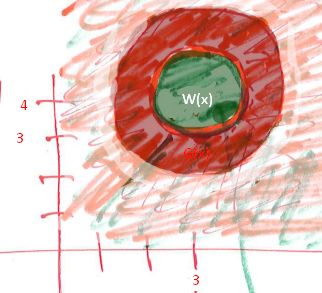
\includegraphics[width=4cm, height=3cm]{pic21}
    \end{itemize}
  \end{itemize}
  \par
\vspace{6mm}
\subsubsection{Exercise 2}
Larry has the utility function $u(x,y)=x^{4}y^{2}$ over two goods whose quantities are denoted by $x \geq 0$ and $y \geq 0$. \par \vspace{0.3em}
  \underline{Are Larry's Preferences complete, transitive, and continuous}?
  \begin{itemize}
    \item  \underline{Answer}: if there is a utility representation of the preferences then the preferences must be complete and transitive (as is the case). Since the utility function is continuous, this implies that the preferences are continuous.
  \end{itemize}
  \par
  \underline{If the price of each good is $1$ per unit and income is $30$, solve for the optimal bundle using the three methods below}?
  \begin{itemize}
    \item  \underline{Indifference and Budget Line Tangency}: Note that since the utility function is smooth (ie twice continuously differentiable), the indifference curves are convex, and monotonicity holds, it follows that interior solutions occur only where the indifference curve of the bundle is tangent to the budget line. This interior solution is captured by the following equations:
    \begin{gather*}
      \frac{MU_{x}}{p_{x}} = \frac{MU_{y}}{p_{y}} \Rightarrow tfrac{4x^{3}y^{2}}{1} = \frac{2x^{4}y}{1} \ \tag{1} \\
      p_{x}x + p_{y}y = I \Rightarrow x + y = 30 \ \tag{2}
    \end{gather*}
    Note that equation (2) puts us on the budget line and equation (1) ensures that trading $x$ for $y$ (and vice versa) will not increase utility. Solving equation (1) yields $2y = x$. By substituting $2y = x$ into equation (2) we get $3y = 30 \ \therefore \ y = 10$. Since $y=10$ we have from equation (2) that $x + 10 = 30$ and therefore $x = 20$. Our optimal bundle is $(x,y) = (20, 10)$
    \item  \underline{Lagrangian}: setting up the lagrangian we have $L = x^{4}y^{2} + \lambda (x + y - 30)$. The partial derivatives of the lagrangian are therefore:
    \begin{gather*}
      \frac{\partial L}{\partial x} = 0 \Rightarrow 4x^{3}y^{2} = \lambda \ \tag{1} \\
      \frac{\partial L}{\partial y} = 0 \Rightarrow 2x^{4}y = \lambda \ \tag{2} \\
      \frac{\partial L}{\partial \lambda} = 0 \Rightarrow x + y - 30 = 0 \ \tag{3}
    \end{gather*}
    From equations (1) and (2) we have:
    \begin{gather*}
      4x^{3}y^{2} = \lambda = 2x^{4}y \\
      \therefore \ y = 0.5x
    \end{gather*}
    Plugging $y = 0.5x$ into equation (3) yields $0.5x + x = 30 \ \therefore \ x = 20$. Substituting $x$ into the budget line yields $y + 20 = 30 \ \therefore \ y = 10$. Our optimal bundle is $(x,y) = (20, 10)$
    \item  \underline{Cobb-Douglass Formula}: the Cobb-Douglas utility function has the general form $u(x,y) = x^{a}y^{b}$. Since our equation mimics this, we have that $a=4$ and $b=2$. This is known to have a solution for all $a,b > 0$ which is given by:
    \begin{gather*}
      x = \frac{aI}{(a+b)p_{x}} = \frac{4(30)}{(2+4)} = 20 \\
      y = \frac{bI}{(a+b)p_{y}} = \frac{2(30)}{(2+4)} = 10
    \end{gather*}
    Thus, our optimal bundle is $(x,y) = (20, 10)$
  \end{itemize}
  \par
\vspace{6mm}
\subsubsection{Exercise 3}
Demand in a market is given by $D(p) = \tfrac{100}{p^{2}}$ for $p > 0$ and the cost of production is $C(Q) = 6 \sqrt{Q} + Q$ \par \vspace{0.3em}
  \underline{Monopoly Market}: suppose we have a monopoly seller. Invert the demand curve and find the monopoly output level $Q$ and the corresponding price level $p$, or argue that one does not exist.
  \begin{itemize}
    \item  \underline{Answer}: inverting the demand function gives $P(Q) = \tfrac{10}{\sqrt{Q}}$. For a monopolist seller the optimal output is given by setting $\text{MR} \ = \ \text{MC}$, so we must first find $MR$ and $MC$:
    \begin{align*}
      &\text{MC} = \frac{\partial C}{\partial Q} = 3Q^{-0.5} + 1 \\
      &\text{MR} = \frac{\partial Q \times P}{\partial Q} = \frac{\partial 10Q^{0.5}}{\partial Q} = 5Q^{-0.5}
    \end{align*}
    Setting $MR = MC$ yields:
    \begin{align*}
      5Q^{-0.5} &= 3Q^{-0.5} + 1 \\
      1 &= Q^{-0.5}(5-3) \\
      Q &= 4
    \end{align*}
    The optimal output $Q = 4$ results in a price of $P = \tfrac{10}{\sqrt{4}} = 5$. Note that this method is valid as the function is concave and allows us to find all interior solutions. As $p$ is restricted to be above zero, and thus $Q$ is restricted to be above zero, we are only dealing with interior points as possible solutions.
    \item  \underline{Alternative Method}: note that we can also insert $P(Q) = \tfrac{10}{\sqrt{Q}}$ into the profit function $\pi = P(Q)Q - C(Q)$, which yields:
    \begin{gather*}
      \pi = \bigg(\frac{10}{\sqrt{Q}} \bigg)Q - (6\sqrt{Q} + Q) = 4\sqrt{Q} - Q
    \end{gather*}
    Taking first order conditions, with respect to $Q$, for profit maximization at an interior point gives us:
    \begin{gather*}
      tfrac{\partial \pi}{\partial Q} = 0 \Rightarrow 2Q^{-0.5} - 1 = 0 \ \therefore \ Q = 4
    \end{gather*}
  \end{itemize}
  \par
  \underline{Competitive Market}: suppose we have sellers in a competitive market. Eithere find a competitive equilibrium or argue that one does not exist.
  \begin{itemize}
    \item  \underline{Answer}: Note that since we have a perfectly competitive market, we take each price as given so $P(Q) = p$ and choose $Q$ to maximize profit. Profit in this case is:
    \begin{gather*}
      \pi = pQ - (6\sqrt{Q} + Q) = Q(p-1) - 6\sqrt{Q}
    \end{gather*}
    While this function is twice continuously differentiable, it is not concave since $\tfrac{\partial^{2}\pi}{\partial Q^{2}} > 0$ making it a strictly convex function. Also note that marginal cost is a decreasing function of output since $\tfrac{\partial^{2}\pi}{\partial Q^{2}} = \tfrac{\partial^{2}C}{\partial Q^{2}} < 0$ (note that the two double derivative are equal due to $P=MC$ in perfect competition). Unlike the case with the monopolist seller, who is able to restrict quantity to increase prices, in a competitive market this is not. Therefore, at $P = MC$ profit will increase with each in output and sellers would never stop producing. As a result there is no competitive equilibrium. To break this down we have the following:
    \begin{itemize}
      \item  \underline{Case (1)}: if $0 < p \leq 1$, then profit is diminishing with quantity. Therefore, each seller would like to supply as little as possible and so market supply is $S(p) = 0$. However, demand would be $D(p) = \tfrac{100}{p^{2}} \geq 100 > 0 = S(p)$. Overall, we would have a case where demand is high but production is nonexistent.
      \item  \underline{Case (2)}: if $p > 1$, then each seller would like to move toward infinite output. This would cause supply to be greater than demand since $D(p) = \tfrac{100}{p^{2}} < 100 < S(p) = +\infty$.
    \end{itemize}
    Overall, in boths case (1) and (2) we do not have a competitive equilibrium.
    \item  \underline{Note}: if trying to solve this at $P=MC$ this will result in $Q=49$ and $P = 1.428$. This yields negative profit where $\pi = Q(p-1) - 6\sqrt{Q} = 49(1.428 - 1) - 6\sqrt{49} = -21.028$. Profit at the competitive equilibrium cannot be equal to zero.
  \end{itemize}
  \par
\vspace{6mm}
\subsubsection{Exercise 3}
Let preferences on a set $X$ be described by a binary relation $\succeq$ which is assumed to be complete and transitive. Let $\sim$ be defined in the standrad way from $\succeq$, that is, $x \sim y$ if and only if $x \succeq y$ and $y \succeq x$. You are goint to help prove that $\sim$ satisfied the following property:
\begin{gather*}
  \forall x,y,z \in X, \ x \sim y \ \text{and} \ y \sim z \ \text{implies} \ x \sim y
\end{gather*}
In your answer, put the completed statement filling in the missing parts
 \par \vspace{0.3em}
  \underline{Question 1}: let \_\_\_\_\_ $\in X$ be given and suppose $x \sim z$ and $y sim z$
  \begin{itemize}
    \item  \underline{Answer}: $x,y,z$
  \end{itemize}
  \par
  \underline{Question 2}: by \_\_\_\_\_, it follows that $y \succeq z$ and $z \succeq x$
  \begin{itemize}
    \item  \underline{Answer}: the definition of indifference
  \end{itemize}
  \par
  \underline{Question 3}: by the result of question 2 and \_\_\_\_\_, it follows that $y \succeq x$
  \begin{itemize}
    \item  \underline{Answer}: transitivity of $\succeq$
  \end{itemize}
  \par
  \underline{Question 4}: use similar arguments as those in questions 1 and 2 to show that $x \succeq y$
  \begin{itemize}
    \item  \underline{Answer}: also by the definition of indifference, it follows that since $x \sim z$ and $y \sim z$ then $z \succeq y$ and $x \succeq z$. By transitivty, we have that $x \succeq y$
  \end{itemize}
  \par
  \underline{Question 5}: give a conclusion statement for your proof
  \begin{itemize}
    \item  \underline{Answer}: we have shown that if $x \sim z$ and $y \sim z$ then by transitivity and the definition of indifference $x \succeq y$ and $y \succeq x$. Since $x \succeq y$ and $y \succeq x$, we have that $x \sim y$. Since $x$, $y$, and $z$ were arbitrarily chose then the property holds
  \end{itemize}

\newpage

\vspace{2.5mm}
\subsection{Quasi-Concavity and Utility Maximization}
In this section we will be focusing on the consumer problem, which is to find an optimal bundle within the consumer's budget. We will first look at conditions that ensure an optimal bundle exists and add the assumption of quasi-concavity of a utility function. This will allow us to use math techniques to solve consumer problems. \par
\vspace{6mm}
\subsubsection{Consumer Problem}
For the standard consumer problem, we will take the consumer to have a budget, $I \in \mathbb{R}_{++}$, and to be able to buy as much of each good as he can afford with his income at fixed positive per unit prices $p = (p_{1}, p_{2}, \dots, p_{n}) \in \mathbb{R}_{++}^{n}$ \par \vspace{0.3em}
\underline{The Consumer's Problem}: to find a bundle $x \in B(p, I)$ such that $x \succeq y$ for all $y \in B(p, I)$, referred to as the optimal bundle \par
\underline{Affordable Bundles}: the consumer's problem allows us to define affordable bundles as those that are in the consumer's budget set where $B(p, I) = \left\{ x \in \mathbb{R}_{+}^{n}: \ p \cdot x \leq I \right\}$
\begin{itemize}
  \item  \underline{Note}: $p \cdot x = \sum_{i=1}^{n}p_{i}x_{i}$
  \item  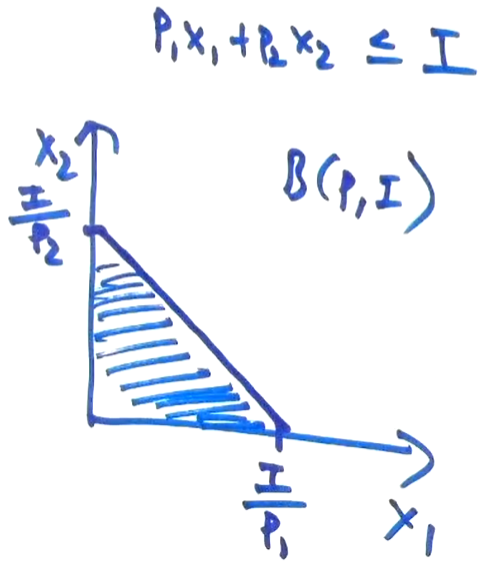
\includegraphics[width=4cm, height=3cm]{pic13}
\end{itemize}
\par
\vspace{6mm}
\subsubsection{Existence of an Optimal Bundle (Weierstrass Theorem)}
Every continuous real-valued function $f$ on a non-empty compact subset $B$ of $\mathbb{R}^{n}$ obtains a maximum on $B$. In otherwords, there is an $x \in B$ such that $f(x) \geq f(y)$ for all $y \in B$ \par \vspace{0.3em}
  \underline{Implication}: therefore, all we need to do is assume the preferences are represented by a continuous utility function and show that the budget set is compact and non-empty to solve the consumer problem \par
  \underline{Requirements}: the budget set is a closed, bounded, and non-empty subset of $\mathbb{R}$
  \begin{itemize}
    \item  \underline{Example}: the budget set figure above is closed, bounded, and non-empty and therefore when alying a continuious real value function to it we will find a maximum
  \end{itemize}
\vspace{6mm}
\subsubsection{Quasi-Concavity}
A real valued function $f$ on $R_{+}^{n}$ is quasi-concave if and only if for all $x, y \in \mathbb{R}_{+}^{n}$ and all $t \in [0,1]$: \\ if $u(x) \geq u(y)$ then $u(tx + (1-t)y) \geq u(y)$ \par \vspace{0.3em}
  \underline{Relationship to Convex Preferences}: quasi-concavity is the translation of convex preferences into a utility representation, if you (don't) have convex preferences then the utility function will (not) be quasi-concave \par
  \underline{Strictly Quasi-Concave}: a real-valued function $f$ on $\mathbb{R}_{+}^{n}$ is strictly quasi-concave if and only if for all distinct $x, y \in \mathbb{R}^{+}_{n}$ and all $t \in (0,1)$: if $u(x) \geq u(y)$ then $u(tx + (1-t)y) > u(y)$
  \par
  \underline{Theorem 1}: every concave function is quasi-concave and every strictly concave function is strictly quasi-concave
  \begin{itemize}
    \item  \underline{Logic}: this result stems from the representation of convex preferences as indifference curves, note that if you draw indifference curves for a quasi-concave function then the indifference curve will be convex
  \end{itemize}
  \par
  \underline{Examples}: (1) is $u(x) = x^{2}$ (strictly) quasi-concave? (2) is $u(x,y) = x^{2} + y$ (strictly) quasi-concave?
  \begin{itemize}
    \item  \underline{Answer 1}: the function is strictly quasi-concave since $y$ always has a lower utility than if the average of $y$ and some higher value $x$. Also note that the set is convex and therefore the function must be quasi-concave. Note that though this is a convex function it is still quasi-concave.
    \begin{itemize}
      \item  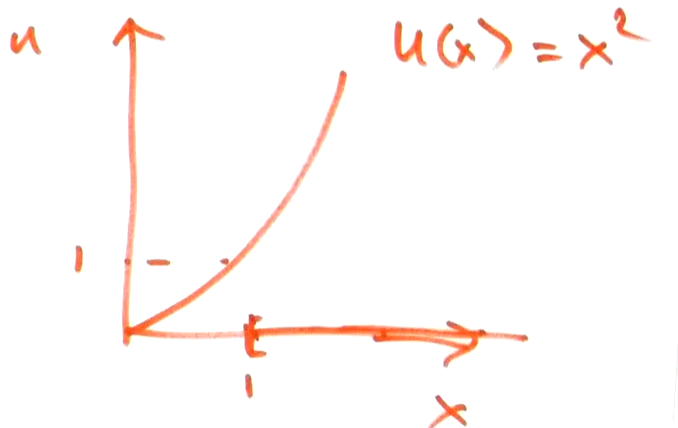
\includegraphics[width=8cm, height=6cm]{pic19}
    \end{itemize}
    \item  \underline{Answer 2}: $u(x,y) = x^{2} + y$ is not a convex set since the better than set is not convex (i.e. drawing a line between two bundles in the better than set would result in points being in the worse than set). Note that in this case averages are not better than extremes in this case, the line in the figure represents an indifference curve. Therefore, the function is not quasi-concave
    \begin{itemize}
      \item  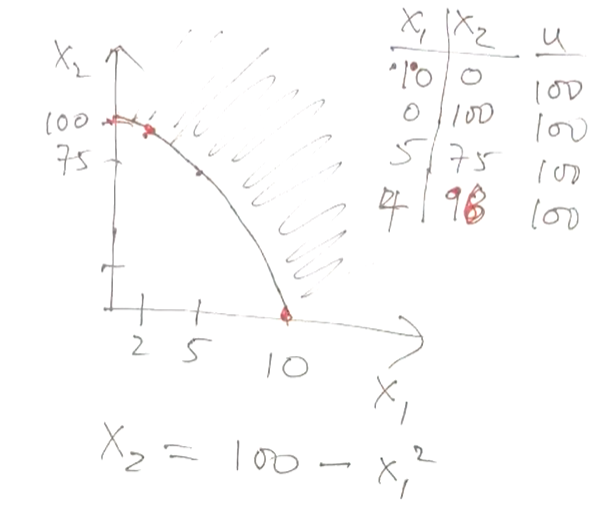
\includegraphics[width=8cm, height=6cm]{pic18}
    \end{itemize}
    You can also demonstrate that this set is not quasi-concave by comparing bundle 1 $(x,y) = (2, 14)$ to bundle 2 $(x,y) = (4, 1)$. In this case, bundle 1 has utility $2^{2} + 14 = 18$ and bundle 2 has utility $4^2 + 1 = 17$, so bundle 1 $\succ$ bundle 2. \\ If we take $t=0.5$ to form a new bundle, i.e. bundle 3 $(tb_{1}x + (1-t)b_{2}x, tb_{1}y + (1-t)b_{2}y) = (3, 7.5)$, then bundle 3 has utility $3^{2} + 7.5 = 16.5$. \\ In this case, bundle 2 $\succ$ bundle 3 and therefore quasi-concavity is violated.
  \end{itemize}
  \par
\vspace{6mm}
\subsubsection{Lagrangian Approach to Bundle Optimality}
If the utility function is continuously differentiable, that is, the partial derivatives are all continuous functions then we can use the Lagrangian Approach to find a solution to the consumer's problem \par \vspace{0.3em}
  \underline{Lagrangian Approach}: set up the Lagrangian where $L(x, \lambda) = u(x) + \lambda (p \cdot x - I)$ and look for solutions $(x^{*}, \lambda^{*})$, where $x_{i}^{*} > 0$ for each good $i$ and $\lambda^{*} > 0$, to the system: \\
  \null\quad (1) $\tfrac{\partial L}{\partial x_{i}} = \tfrac{\partial u(x^{*})}{\partial x_{i}} - \lambda^{*}p_{i}$ \quad for each $i = 1, \dots, n$ where you have $n$ equations \\
  \null\quad (2) $\tfrac{\partial L}{\partial \lambda} = p \cdot x - I = 0$
  \par
  \underline{Sufficiency of the Lagrangian Method}: if $u(x)$ is continuously differentiable, stricty monotonic, and quasi-concave, then any solution to the Lagrangian approach is a solution to the consumer's problem
  \begin{itemize}
    \item  \underline{Logic}: system equation (1) implies \textit{equalization of bang for buck} where for any two goods $i$ and $j$ we have $$\frac{\tfrac{\partial u(x^{*})}{\partial x_{i}}}{p_{i}} = \frac{\tfrac{\partial u(x^{*})}{\partial x_{j}}}{p_{j}}$$ System equation (2) implies budget exhausted, i.e. that the optimal bundle is on the budget line
    \begin{itemize}
      \item  \underline{Bang for Buck across Goods}: this is a multi-dimensional version of do it until the \textit{marginal benefit equals marginal cost} (i.e. marginal gain equals marginal pain). This is your point of tangency between the budget set and the indifference curve
    \end{itemize}
  \end{itemize}
  \par
  \underline{Bang-for-Buck}: we can use bang-for-buck directly without using the full lagrangian method where we find a solution using $\frac{\tfrac{\partial u(x^{*})}{\partial x_{i}}}{p_{i}} = \frac{\tfrac{\partial u(x^{*})}{\partial x_{j}}}{p_{j}}$ and $p \cdot x = I$
  \par
  \underline{Uniqueness of Solution}: if $u(x)$ is strictly quasi-concave, then there is at most one solution to the consumer's problem. Note that for cases of non-strictly quasi-concave preferences, we can have more than one solution (i.e. if you have perfect substitutes)
  \par
  \underline{Example}: for $u(x_{1},x_{2}) = x_{1}x_{2}$ where $p_{1} = 10$, $p_{2} = 5$, and $I = 50$ we set up the lagrangian as $L = x_{1}\cdot x_{2} - \lambda(10x_{1} + 5x_{2} - 50)$. The system of equations is given by:
  \begin{align*}
    &\frac{\partial L}{\partial x_{1}} = 0 \Rightarrow x_{2} - 10\lambda = 0 \ \therefore \ \lambda = \frac{x_{2}}{10} \ \tag{1} \\
    &\frac{\partial L}{\partial x_{2}} = 0 \Rightarrow x_{1} - 5\lambda = 0 \ \therefore \ \lambda = \frac{x_{1}}{5} \ \tag{2} \\
    &\frac{\partial L}{\partial \lambda} = 0 \Rightarrow 10x_{1} + 5x_{2} - 50 = 0 \ \tag{3}
  \end{align*}
  Setting equations (1) and (2) equal to eachother yields:
  \begin{gather*}
    \frac{x_{2}}{10} = \lambda = \frac{x_{1}}{5} \\
    x_{2} = 2x_{1}
  \end{gather*}
  Subtituting $x_{2} = 2x_{1}$ into equation (3) gives us $10x_{1} + 5(2x_{1}) = 50 \ \therefore \ x_{1} = 2.5$. Since $x_{1} = 2.5$ we have that $x_{2} = 2x_{1} = 5$. Note that $\lambda > 0$ since $\lambda = \tfrac{x_{2}}{10} = 0.5$, making the solution valid. Our optimal bundle is therefore $(x_{1}, x_{2}) = (2.5, 5)$
  \par
\vspace{6mm}
\subsubsection{Exercise 1}
Let Jane have the utility function $u(x,y) = 2x + \ln y$ \par \vspace{0.3em}
\begin{itemize}
  \item  \underline{Question 1}: find the optimal demands for Jane using the Lagrangian method if income $I = 10$ and prices are $p_{x} = 1$ and $p_{y} = 2$
  \begin{itemize}
    \item  \underline{Answer}: our lagrangian equation is
    \begin{gather*}
      \mathcal{L} = 2x + \ln(y) + \lambda (p_{x} x + p_{y}y - I)
    \end{gather*}
    From this we derive the following first order conditions:
    \begin{align*}
      0 = \tfrac{\partial \mathcal{L}}{\partial x} &= 2 + \lambda p_{x} \Rightarrow -\lambda = \frac{2}{p_{x}} \ \tag{1} \\
      0 = \frac{\partial \mathcal{L}}{\partial y} &= \frac{1}{y} + \lambda p_{y} \Rightarrow - \lambda = \tfrac{1}{yp_{y}} \ \tag{2} \\
      0 = \frac{\partial \mathcal{L}}{\partial \lambda} &= p_{x}x + p_{y}y - I \ \tag{3}
    \end{align*}
    Setting equation $(1)$ equal to $(2)$ we can solve for $y$:
    \begin{align*}
      \tfrac{2}{p_{x}} &= \tfrac{1}{y p_{y}} \\
      2y p_{y} &= p_{x} \ \tag{4} \\
      \therefore y &= \tfrac{p_{x}}{2p_{y}} \ \tag{*}
    \end{align*}
    Substituting $(*)$ into equation $(3)$ we can solve for $x$:
    \begin{align*}
      p_{x}x + p_{y}(\tfrac{p_{x}}{2p_{y}}) &= I \\
      p_{x}x + \frac{p_{x}}{p_{y}} &= I \\
      \therefore x &= \frac{I}{p_{x}} - \frac{1}{p_{y}} \ \tag{**}
    \end{align*}
    Not that by substituting $(*)$ into $(4)$, we can find when spending on both $x$ and $y$ is not optimal:
    \begin{gather*}
      P_{y}(\frac{p_{x}}{2p_{y}}) = \frac{p_{x}}{2} > I \ \tag{***}
    \end{gather*}
    This result arises since $\lim_{y \rightarrow 0} \ln(y) = -\infty$, so if $(***)$ occurs then everything is spent on $y$. This yields the following solution:
    \begin{gather*}
      y =
      \begin{cases}
        \frac{p_{x}}{2p_{y}} & \text{ if } \frac{P_{x}}{2} \leq I \\
        \frac{I}{p_{y}} & \text{ if } \frac{p_{x}}{2} > I
       \end{cases}
      \\
      x =
      \begin{cases}
        \frac{I}{p_{x}} - \frac{1}{p_{y}} & \text{ if } \frac{p_{x}}{2} \leq I \\
        0 & \text{ if } \frac{p_{x}}{2} > I
       \end{cases}
    \end{gather*}
    Using $I = 10$, $p_{x} = 1$, and $p_{y} = 2$ we have the $\tfrac{p_{x}}{2} < I$, giving us the optimal bundle $y = 0.25$ and $x = 10 - 0.5 = 9.5$
  \end{itemize}
  \item  \underline{Question 2}: find the optimal demands for Jane when $I = 10$ and prices are $p_{x} = 8$ and $p_{y} = 2$
  \begin{itemize}
    \item  \underline{Answer}: Using $I = 10$, $p_{x} = 8$, and $p_{y} = 2$ we have the $\tfrac{p_{x}}{2} < I$, giving us the optimal bundle $y = 2$ and $x = 10/8 - 0.5 = 0.75$
  \end{itemize}
\end{itemize}
\par
\vspace{6mm}
\subsubsection{Exercise 2}
Let $u(x,y) = x^{2} + y^{2}$ \par \vspace{0.3em}
\begin{itemize}
  \item  \underline{Question 1}: use the bundles $(5,0)$ and $(0,4)$ to show that these preferences are not strictly convex
  \begin{itemize}
    \item  \underline{Answer}: preferences are convex if and only if for all $x,y \in R_{n}^{+}$ and all $t \in [0,1]$, if $x \succeq y$ then $tx + (1-t)y \succeq y$.\\ For bundle 1 we have $(x,y) = (5,0)$ with utility $u  = 5^{2} + 0 = 20$. For bundle 2 we have $(x,y) = (0,4)$ with utility $u = 0 + 4^{2} = 16$. Therefore bundle 1 $\succ$ bundle 2.\\ If we take $t=0.5$ to form a new bundle, i.e. bundle 3 $(x,y) = (tb_{1} x + (1-t)b_{2}x, tb_{1}y + (1-t)b_{2}y) = (2.5, 2)$, then bundle 3 has utility $u = 2.5^{2} + 2^{2} = 10.5$.\\ In this case bundle 2 $\succ$ bundle 3 and so preferences are not convex.
  \end{itemize}
  \item  \underline{Question 2}: why does the lagrangian method fail here?
  \begin{itemize}
    \item  \underline{Answer}: since preferences are not convex we have that $u(x)$ is not quasi-concave. This violates the quasi-concavity sufficient condition for the lagrange method
  \end{itemize}
  \item  \underline{Question 3}: what is an optimal bundle if $I=10$ and prices are $p_{x}=1$ and $p_{y} = 2$
  \begin{itemize}
    \item  \underline{Answer}: since $u(x, y) = x^{2} + y^{2}$, utility is maximized by spending all $I$ on the cheapest good. In other words, we have that:
    \begin{gather*}
      x =
      \begin{cases}
        \frac{I}{p_{x}} & \text{ if } p_{x}<p_{y} \\
        0 & \text{ if } p_{x} > p_{y} \\
        \frac{I}{p_{x}} &  \text{ if } p_{x} = p_{y} \textit{ and } y = 0
       \end{cases}
      , \ \ \
      y =
      \begin{cases}
        0 & \text{ if } p_{x}<p_{y} \\
        \frac{I}{p_{y}} & \text{ if } p_{x} > p_{y} \\
        \frac{I}{p_{y}} &  \text{ if } p_{x} = p_{y} \textit{ and } x = 0
       \end{cases}
    \end{gather*}
    Therefore, for $I=10$, $p_{x} = 1$, and $p_{y} = 2$, the optimal bundle is $(x, y) = (10, 0)$
  \end{itemize}
\end{itemize}
\par
\vspace{6mm}
\subsubsection{Exercise 3}
Consider a utility representation $u(x,y) = v(x) + y$ where $v$ is a function that does not depend on $y$/ Argue that this utility function is quasi-concave if $v(x)$ is concave\par \vspace{0.3em}
\begin{itemize}
  \item  \underline{Answer}: for a quasi-linear utility function $u(x,y) = v(x) + y$ to be quasi-concave we need that both $v(x)$ and $y$ are concave.\\ Supposing that $v(x)$ is concave we must show that $y$ is concave, $y$ must be concave since it is strictly monotonic and therefore for all $t \in [0,1]$ and $\forall y_{1},y_{2} \in \mathbb{R}$ we have that $u(ty_{1} + (1-t)y_{2}) \geq tu(y_{1}) + (1-t)u(y_{2})$.\\ Since the sum of concave functions is concave this means that $u(x,y) = v(x) + y$ is concave, Since a concave function is quasi-concave, we have that $u(x,y)$ is quasi-concave
  \item  \underline{Alternative Answer}: suppose $v(x)$ is concave, we need to show that $u(x,y)$ is quasi-concave.\\ Quasi-concavity is when for all $t \in [0,1]$ if $u(x,y) \geq u(x',y')$ then $u(tx + (1-t)x', ty + (1-t)y') \geq u(x', y')$.\\ Note that in this case $u(tx + (1-t)x', ty + (1-t)y') = v(tx + (1-t)x') + (ty + (1-t)y')$ and, since $V(x)$ is concave, by definition:
  \begin{gather*}
    v(tx + (1-t)x') + (ty + (1-t)y') \geq tv(x) + (1-t) v(x') + ty + (1-t)y' \ \tag{1}
  \end{gather*}
  The RHS of equation $(1)$ can be rewritten as: $t(v(x) + y) + (1-t)(v(x')+y') = tu(x,y) + (1-t)u(x',y')$. Thus, we have that
  \begin{gather*}
    u(tx + (1-t)x', ty + (1-t)y') \geq tu(x,y) + (1-t)u(x',y') \ \tag{2}
  \end{gather*}
  Since $u(x,y) \geq u(x',y')$ it follows that $tu(x,y) + (1-t)u(x',y') \geq u(x',y')$. Combining this result with $(2)$ we therefore have that $u(tx + (1-t)x', ty + (1-t)y') \geq tu(x,y) + (1-t)u(x',y') \geq u(x', y')$, so $u(x,y)$ is quasi-concave
\end{itemize}
\par
\vspace{6mm}
\subsubsection{Exercise 4}
Argue formally that the budget set defined as a subset of $\mathbb{R}_{+}^{n}$ is convex for positive prices and income \par \vspace{0.3em}
\begin{itemize}
  \item  \underline{Answer}: suppose $p > 0$ and $I > 0$, we need to show that the budget set $B(p,I) = \left\{ x \in R^{+}_{n}: px \leq I \right\}$ is convex.\\ We have that $B(p, I)$ is convex if for all $x,y \in B(p,I)$ for all $t \in [0,1]$:
  \begin{gather*}
    tx + (1-t)y \in B(p, I)
  \end{gather*}
  Since $x, y \in B(p, I)$ it follows that $px \leq I$ and $py \leq I$. Therefore, using $t$, we have:
  \begin{align*}
    ptx &\leq tI \ \tag{1} \\
    p(1-t)y &\leq (1-t)I \ \tag{2}
  \end{align*}
  Summing equations $(1)$ and $(2)$ yields:
  \begin{gather*}
    p(tx + (1-t)y) \leq I \ \tag{3}
  \end{gather*}
  Equation $(3)$ takes the same form as our definition for $B(p,I)$ and so we have that:
  \begin{gather*}
    B(p,I) = \left\{ tx + (1-t)y \in R_{n}^{+}: p(tx + (1-t)y) \leq I \right\}
  \end{gather*}
  Therefore, $tx + (1-t)y \in B(p, I)$
\end{itemize}
\par
\vspace{6mm}
\subsubsection{Exercise 5}
Let $X$ be a convex subset of $\mathbb{R}_{+}^{n}$. We say that $x \in X$ \textit{maximizes u over $X$ if and only if $u(x) \geq u(y)$ for all $y \in X$}. \par \vspace{0.3em}
\begin{itemize}
  \item  \underline{Question 1}: prove that if $u$ is quasi-concave, then the set $M(X) = \left\{ x \in X: x \ \textit{maximizes} \ u \ \textit{over} \ X \right\}$ is a convex set
  \begin{itemize}
    \item  \underline{Answer}: We must show that $M(x)$ is convex. Note that we can rewrite $M(X) = \left\{ x \in X: x \ \textit{maximizes} \ u \ \textit{over} \ X \right\}$ as follows:
    \begin{gather*}
      M(X) = \left\{x \in X: u(x) \geq u(y), \ \forall y \in X \right\} \ \tag{1}
    \end{gather*}
    Suppose that $u$ is quasi-concave whereby if $u(x) \geq u(y)$ then for all $t = [0,1]$ we have $u(tx + (1-t)y) \geq u(y)$. From this, definition (1) can be rewritten as
    \begin{gather*}
      M(X) = \left\{x \in X: u(tx + (1-t)y) \geq u(y), \ \forall y \in X, \forall t \in [0,1] \right\} \ \tag{2}
    \end{gather*}
    Using proof by contradiction, suppose that $X$ is \textbf{not} convex wherein for some $x,y \in M(X)$ and for some $t \in [0,1]$:
    \begin{gather*}
      y \succ tx + (1-t) y
    \end{gather*}
    This would mean that:
    \begin{gather*}
      M(X) = \left\{x \in X: u(y) \geq u(tx + (1-t)y), \ \text{for some } y \in X, \ \text{for some} \ t \in [0,1] \right\}
    \end{gather*}
    which violates definition (2) and the quasi-concavity of $u$. Therefore, by contradiction, $X$ must be convex
  \end{itemize}
  \item  \underline{Question 2}: prove that if $u$ is strictly quasi-concave, then the set $M(X)$ has at most one point
  \begin{itemize}
    \item  \underline{Answer}: if $u$ is strictly quasi-concave then defintion (2) becomes:
    \begin{gather*}
      M(X) = \left\{x \in X: u(tx + (1-t)y) > u(y) ,\ \forall y \neq x \in X, \forall t \in (0,1) \right\} \ \tag{3}
    \end{gather*}
    Since $X$ is convex we have that for all $x, y \in X$ and for all $t \in [0,1]$: $tx + (1-t)y \succeq y$. \\
    In the case where $tx + (1-t)y \sim y$ we would have that $u(tx + (1-t)y) = u(y)$, contradicting definition $(3)$. Therefore, we must have strict convex preferences wherein for all $x, y \in \mathbb{R}$ and for all $t \in [0,1]$: $tx + (1-t)y \succ y$. In otherwords, we must have no bundles that are valued indifferently and therefore there must exist a bundle that is strictly preferred to all other bundles. Thus, the set $M(X)$ has at most one point.
  \end{itemize}
  \item  \underline{Question 3}: do we need $u$ to be continuous for the results from questions 1 and 2 to hold
  \begin{itemize}
    \item  \underline{Answer}: no, since the results are about the \textit{set of maximizers} ina a convex set. They hold whether or not the \textit{set of maximizers} is empty. The empty set is convex and has at most one point since it has no point
  \end{itemize}
\end{itemize}
\par
\vspace{6mm}
\subsubsection{Exercise 6}
Rick has the following utility function:
\begin{gather*}
  u(x,y) =
  \begin{cases}
    x & \text{ if } y > x \\
    y & \text{ if } y < x \\
    0 & \text{ if } x = y
   \end{cases}
\end{gather*}
\par \vspace{0.3em}
\begin{itemize}
  \item  \underline{Question 1}: Argue that Rick's preferences are not continuous
  \begin{itemize}
    \item  \underline{Answer}: consider the set $(x,y) = (9,9)$ with $f(9,9) = 0$. For preferences to be continuous at $(x,y) = (9,9)$ then every sequence that converges to $(9,9)$ must also converge to in the codomain to $f(9,9)$.\\ Using the sequence $\lim_{n \rightarrow \infty} (9 - \tfrac{1}{n}, 9)$ we have that at $\lim_{n \rightarrow \infty} f(9 - \tfrac{1}{n}, 9) = 0$. However, for all $N < \infty$ we have that $\lim_{n \rightarrow N} f(9 - \tfrac{1}{n}, 9) = 9$. Therefore, convergence is violated as there no $n$'s such that for $\varepsilon < 9$ the following holds:
    \begin{gather*}
      \forall \varepsilon > 0 \exists N \in \mathbb{N} \forall n \geq N: |x_{n} - x^{*}| < \varepsilon
    \end{gather*}
    Note that in this case we have:
    \begin{gather*}
      |(9 - \frac{1}{n}, 9) - (9, 9)| = |9 - 0| = 9 > \varepsilon \forall \varepsilon \leq 9
    \end{gather*}
  \end{itemize}
  \item  \underline{Question 2}: suppose that Rick's utility function changes to
  \begin{gather*}
    u(x,y) =
    \begin{cases}
      x & \text{ if } x \in [0,10] \\
      2x & \text{ if } x > 10
     \end{cases}
  \end{gather*}
  are his preferences continuous now?
  \begin{itemize}
    \item  \underline{Answer}: consider the sequence $\lim_{n \rightarrow \infty} (10 + \tfrac{1}{n})$. We have that the codomain at this limit is $\lim_{n \rightarrow \infty} f(10 + \tfrac{1}{n}) = 10$. However, for $N < \infty$ we have that $\forall n \in N: f(10 + \tfrac{1}{n}) = 2(10 + \tfrac{1}{n})$. Therefore, the preferences are not continuous since convergence does not hold since:
    \begin{gather*}
      |x_{n} - x^{*}| = |2(10 + \frac{1}{n}) - 10| = 10 + \frac{2}{n} < \varepsilon
    \end{gather*}
  \end{itemize}
\end{itemize}

\newpage

\vspace{2.5mm}
\subsection{Demand and Consumer Welfare}
Unlike previous sections, this section will be focusing on the total demand and consumer welfare instead of the demand of an individual consumer. \par
\vspace{6mm}
\subsubsection{Demand}
Demand of each good depends on potentially all prices and income. We write $x(p,I)$ to denote a bundle that maximizes utility subject to the budget constraint. This bundle $x(p,I)$ (or bundles) is called the demand at prices and income $(p, I)$  \par \vspace{0.3em}
  \underline{Demand Function}: a demand function assigns a bundle/s $x(p, I)$ to each budget $(p,I)$
  \begin{itemize}
    \item  \underline{Conditions for Uniqueness}: if utility is strictly quasi-concave, therefore making the budget set convex, we get a unique demanded bundle for each budget that allows us to derive a demand function
    \begin{itemize}
      \item  \underline{Note}: we will not have a unique demanded bundle if we have perfect substitutes (in this case utility won't be strictly quasi-concave) or other functions like $u(x) = x^{2} + y^{2}$ where price is $1$ for both. In this case, while demand cannot be a function, we can still analyze demand and properties of it
    \end{itemize}
    \item  \underline{Relationship with Utility Functions}: if utility functions are differentiable and strictly convex, the demand functions will often be as well. In such cases, we can use partial derivatives to determine how prices and income affect demand for each good
  \end{itemize}
  \par
  \underline{Cobb-Douglas Example}: suppose $u(x) = \prod_{j=1}^{n} x_{j}^{\alpha_{j}}$ where $\alpha_{j} > 0$ for all $j = 1, \dots, n$ and $\sum_{j=1}^{n} \alpha_{j} = 1 \equiv \alpha$, the demands are:
  \begin{gather*}
    x_{i}(p,I) = \frac{\alpha_{i} I}{(\sum_{j=1}^{n}\alpha_{j})p_{i}}
  \end{gather*}
  \par
  \begin{itemize}
    \item  \underline{Properties}: is strictly quasi-concave, since it is the product of the quantities you will never have a quantity equal to zero so you will always consume on the interior, the function is differentiable so we can use lagrange techniques (which yields the above)
    \item  \underline{Incorporating Assumptions}: we can take our utility function and raise it to the power of $\tfrac{1}{\alpha}$ to yield:
    \begin{gather*}
      u(x) = (\prod_{j=1}^{n} x_{j}^{\alpha_{j}})^{\tfrac{1}{\alpha}}, \ \alpha_{j} > 0
    \end{gather*}
  \end{itemize}
  \par
  \underline{Perfect Substitutes Example}: suppose $u(x) = \sum_{j=1}^{n}  x_{j}\frac{\alpha_{j}I}{p_{j}}$, the demands are:
  \begin{gather*}
    x_{i}(p,I) =
    \begin{cases}
     & 0 \text{ if } p_{i} \ \text{is not the lowest price;} \\
     & \tfrac{I}{p_{i}} \text{ if } p_{i} \ \text{is the unique lowest price;} \\
     & \text{non-unique otherwise}
    \end{cases}
  \end{gather*}
  \par
  \begin{itemize}
    \item  \underline{Properties}: preferences are not strictly convex, you can have solutions if there are two or more goods with the same lowest price (i.e. goods are extremely price elastic), utility is quasi-concave
  \end{itemize}
  \par
  \begin{itemize}
    \item  \underline{Note}: this is as the consumer will exhaust all his income one the cheapest good since all good are of equal value to him (i.e. they are perfect substitutes)
  \end{itemize}
  \par
  \underline{Perfect Complements Example}: suppose $u(x) = \min \left\{x_{1}, \dots, x_{n} \right\}$, the demands are:
  \begin{gather*}
    x_{i}(p,I) = \frac{I}{\sum_{j=1}^{n}p_{j}}
  \end{gather*}
  \par
  \begin{itemize}
    \item  \underline{Properties}: given that only the minimum amount of a good counts towards your utility then you will want to have an equal amount of each good - yielding the above demand function
  \end{itemize}
  \underline{Graphic Representation of Examples}: the below figure shows the indifference curves for the above demand function examples \\
  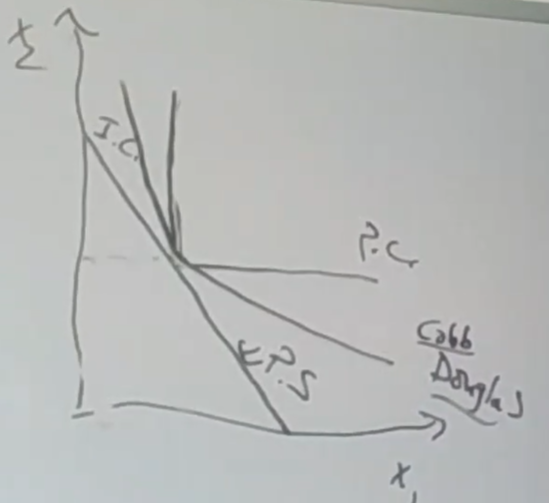
\includegraphics[width=5cm, height=5 cm]{pic23}
  \par
\vspace{6mm}
\subsubsection{Quasi-Linear Utility Functions}
 suppose $u(x) = v(x_{1}) + x_{2}$ where $v(x_{1})$ does not depend on $x_{n}$. In this case, the demand for good 1 will not depend on income (provided income is sufficiently large and the solution is not a corner) \par \vspace{0.3em}
  \underline{Logic}: good 1 is said to have \textit{no-income effects} while good 2 is often taken to be \textit{everything else} with a price of \$1 per unit
  \par
  \underline{Advantage}: this makes consumer welfare easy to estimate as now it is just the area under the demand curve
  \par
  \underline{Linear Demand}: a quadratic function for $v(x_{1})$ would generate a linear demand for $x_{1}$ (i.e. $v(x_{1}) = ax_{1} - bx_{1}^{2}$)
  \par
  \underline{Note}: for a quasi-linear utility function to also be strictly quasi-concave, it is necessary and sufficient that $v$ be quasi-concave. For utility that has a quasi-linear form, so long as $v(x)$ is concave then the preferences will be convex
  \par
\vspace{6mm}
\subsubsection{Indirect Utility Function}
Given that utility is a function of bundles of goods, if a consumer is presumed to choose a bundle that maximizes utility, then we can plug the maximizing bundle $x(p,I)$ into the utility function to get what we call an indirect utility function $v(p,I)$ \par \vspace{0.3em}
  \underline{Mathematic Definition}: $v(p,I) = \max \left\{U(x) | px \leq I \right\}$
  \begin{itemize}
    \item  \underline{Note}: in other words, the indirect utility function is a function/formula that solves the utility function given the utility functions constraints
  \end{itemize}
  \par
  \underline{Non-Unique Bundles}: we do not need to have a unique bundle as a solution since all the best bundles will generate the same utility
  \par
  \underline{Theorem 1}: if $u(x)$ is a continuous and strongly monotonic real valued utility function on $\mathbb{R}_{+}^{n}$, then the indirect utility function $v(p, I)$ is:
  \begin{itemize}
    \item  \underline{(1)}: continuous
    \item  \underline{(2)}: homogeneous of degree zero
    \item  \underline{(3)}: strictly increase in $I$ and weakly increasing in $p$
    \item  \underline{(4)}: the function $f(p, I) = -v(p,I)$ is quasi-concave in $(p,I)$
  \end{itemize}
  \par
  \underline{Roy's Identity}: if $u(x)$ is differentiable and the partial derivative with respect to $I$ is non-zero at a point $(p, I)$ then it satisfies:
  \begin{gather*}
    x_{i}(p, I) = -\frac{\tfrac{\partial v(p,I)}{\partial p_{i}}}{\tfrac{\partial v(p,I)}{\partial I}}
  \end{gather*}
  which allows you to use the indirect utility function to recover demand
  \par
  \underline{Marshallian Demand Function}: a Marshallian demand function gives you the value of $x_{i}$ as a function of its price and income parameters $p_{i}$ and $I$, written as $x_{i}(p,I)$
  \begin{itemize}
    \item  \underline{Logic}: the Marshallian demand function gives the demand for a good given the price of the good and income, which is shown in the below graph where the price of good 1 changes from $p_{1}^{0}$ to $p_{1}^{1}$ where $p_{1}^{0} > p_{1}^{1}$ and so since income does not change we have greater demand for $x_{1}$
    \\
    \begin{center}
      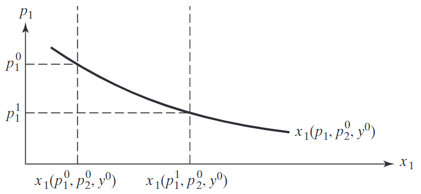
\includegraphics[width=8cm, height=6cm]{pic25}
    \end{center}
  \end{itemize}
  \par
  \underline{Example - Cobb Douglas $n=2$}: the indirect utility function for Cobb-Douglas, $u = x_{1}x_{2}$ where demand is $x_{1} = \tfrac{I}{2p_{1}}$ and $x_{2} = \tfrac{I}{2p_{2}}$, is $V(p,I) = \tfrac{I^{2}}{4p_{1}p_{2}}$
  \begin{itemize}
    \item  \underline{Logic}: this comes from substituting the demand for $x_{1}$ and $x_{2}$ into the utility function, giving us an indirect utility function that yield maximum utility
    \item  \underline{Properties}: the indirect utility function is continuous, strictly increasing in $I$, strictly decreasing in $p$, and strictly monotonic
  \end{itemize}
  \underline{Example - Cobb Douglas $n>2$}: suppose we have $u(x) = \prod_{j=1}^{n} x_{j}^{\alpha_{j}}$ where $\alpha_{j} > 0$ for all $j = 1, \dots, n$ and $\sum_{j=1}^{n} \alpha_{j} = 1 \equiv \alpha$. We want to solve $\max_{x} u(x) \ \text{s.t.} \ \sum_{j=1}^{n}p_{j}x_{j} \leq I$. Since we have strong monotonicity we will always exhaust the budget so our constraint can be rewritten as $\sum_{j=1}^{n}p_{j}x_{j} = I$. We can use bang-for-buck equalization and budget exhaustion to solve this where:
  \begin{gather*}
    \frac{MU_{i}}{p_{i}} = \frac{MU_{j}}{p_{j}}, \ \forall i,j \ \tag{1} \\
    \sum_{j=1}^{n}p_{j}x_{j} = I \ \tag{2}
  \end{gather*}
  Using bang-for-buck equation (1) from the reference point of good 1, we have:
  \begin{align*}
    \frac{MU_{1}}{p_{1}} &= \frac{MU_{j}}{p_{j}} \\
    \frac{\alpha_{1}x_{1}^{\alpha_{1}-1} \prod_{k \neq 1}^{n} x_{k}^{\alpha_{k}}}{p_{1}} &= \frac{\alpha_{j}x_{j}^{\alpha_{j}-1} \prod_{k \neq j}^{n} x_{k}^{\alpha_{k}}}{p_{j}} \\
  \end{align*}
  We want to rearrange the above such that we have $x_{j} = f(x_{1})$. Note that we have positive amounts of all $x_{i}$ due to the multiplication in cobb-douglas and the assumption that $I > 0$. Here we can expand and then cancel out all the $j \neq k$ and $j \neq 1$ to yield:
  \begin{gather*}
    \frac{\alpha_{1}x_{1}^{\alpha_{1} - 1} x_{j}^{\alpha_{j}} \big( \prod_{k \neq j,1}^{n} x_{j}^{\alpha_{k}} \big) }{p_{1}} = \frac{\alpha_{j}x_{j}^{\alpha_{j}-1} x_{1}^{\alpha_{1}} \big( \prod_{k \neq j,1}^{n} x_{k}^{\alpha_{k}} \big)}{p_{j}}
  \end{gather*}
  We can cancel out our summations, $\alpha_{j}$, and $\alpha_{1}$ factors as follows:
  \begin{align*}
    \frac{\alpha_{1}x_{1}^{\alpha_{1} - 1} x_{j}^{\alpha_{j}}}{p_{1}} &= \frac{\alpha_{j}x_{j}^{\alpha_{j}-1} x_{1}^{\alpha_{1}}}{p_{j}} \\
    \frac{\alpha_{1}x_{1}^{\alpha_{1} - 1}}{p_{1}} &= \frac{\alpha_{j}x_{j}^{-1} x_{1}^{\alpha_{1}}}{p_{j}} \\
    \frac{\alpha_{1}x_{1}^{-1}}{p_{1}} &= \frac{\alpha_{j}x_{j}^{-1}}{p_{j}} \ \tag{3}
  \end{align*}
  We can now rearrange equation $(3)$ for $x_{j} = f(x_{1})$:
  \begin{gather*}
    x_{j} = \frac{\alpha_{j}}{\alpha_{1}}\frac{p_{1}}{p_{j}}x_{1} \ \tag{*}
  \end{gather*}
  We can substitute $(*)$ into the budget exhaustion equation $(2)$ and cancel out $p_{i}$'s to yield:
  \begin{align*}
    \sum_{j=1}^{n}p_{i}x_{i} &= I \\
    p_{1}x_{1} + p_{2}\frac{\alpha_{2}}{\alpha_{1}}\frac{p_{1}}{p_{2}}x_{1} + \dots + p_{n}\frac{\alpha_{n}}{\alpha_{1}}\frac{p_{1}}{p_{n}}x_{1} &= I \\
    p_{1}x_{1} + \frac{\alpha_{2}}{\alpha_{1}}p_{1}x_{1} + \dots + \frac{\alpha_{n}}{\alpha_{1}}p_{1}x_{1} &= I \\
    x_{1}\frac{p_{1}}{\alpha_{1}} (\alpha_{1} + \alpha_{2} + \dots + \alpha_{n}) &= I \ \tag{4}
  \end{align*}
  Since $\sum_{j=1}^{n} \alpha_{j} = 1$ we can rewrite equation $(4)$ and solve it for $x_{1}$:
  \begin{align*}
    x_{1}\frac{p_{1}}{\alpha_{1}} &= I \\
    x_{1} &= \frac{\alpha_{1}I}{p_{1}} \ \tag{**}
  \end{align*}
  We can substitute our formula $(**)$ for $x_{1}$ into our formula $(*)$ for $x_{j}$ to solve for $x_{j}$ as a function of known parameters:
  \begin{align*}
    x_{j} &= \frac{\alpha_{j}}{\alpha_{1}}\frac{p_{1}}{p_{j}} \times \frac{\alpha_{1}I}{p_{1}} \\
    x_{j} &= \frac{\alpha_{j}I}{p_{j}} \ \tag{***}
  \end{align*}
  Our indirect utility function is therefore the product of our optimal $x_{j}$'s, given by $(***)$, to the power of $\alpha^{j}$:
  \begin{align*}
    v(p,I) &= max \left\{ u(x)|px \leq I \right\} \\
    v(p,I) &= \prod_{i=1}^{n} (\frac{\alpha_{j}I}{p_{j}})^{\alpha_{j}}  \\
    v(p,I) &= I \prod_{i=1}^{n} (\frac{\alpha_{j}}{p_{j}})^{\alpha_{j}} \ \tag{****}
  \end{align*}
  Note that we raise $x_{j}$ by $\alpha_{j}$ since this is the utility obtained from a given quantity of $x_{j}$. We also can place $I$ outside of $\prod$ since the sum of $\alpha_{j}$ is 1 and $I$ is a constant, i.e. $I^{\alpha_{1}} \times \dots \times I^{\alpha_{n}} = I^{\alpha_{1} + \dots + \alpha_{n}} = I$.
  \par
\vspace{6mm}
\subsubsection{Expenditure Minimization Problem}
Involves finding $x(p, \overline{u})$ to minimize the expenditure $e(p,\overline{u}) = \sum_{i=1}^{n}p_{i}x_{i}$ incurred to obtain utility $\overline{u}$ \par \vspace{0.3em}
\vspace{6mm}
  \underline{Translation}: what is the cheapest way to get a specified level of utility given price and income $(p, I)$
  \par
  \underline{Solution}: solving e-min can be done in the differentiable case using Lagrangian type methods. Note that under standard assumptions of quasi-concave utility, strong monotonicity and interior solution it satisfies bang for buck equalization (MRS equal price ratio) and utility is just equal to $\overline{u}$
  \par
  \underline{Theorem 1}: if $u(x)$ is a continuous and strongly monotonic real valued utility function on $\mathbb{R}_{+}^{n}$ then the expenditure funtion $e(p, \overline{u})$ is:
  \begin{itemize}
    \item  \underline{(1)}: continuous
    \item  \underline{(2)}: homogeneous of degree one in $p$
    \item  \underline{(3)}: strictly increasing in $\overline{u}$ and weakly increasing in $p$
    \item  \underline{(4)}: concave in $p$
  \end{itemize}
  \par
  \underline{Shephard's Lemma}: when $e(p,u)$ is differentiable in $p$ at $(p^{0}, u^{0})$ we have that
  \begin{gather*}
    x_{i}^{h}(p^{0},u^{0}) = \frac{\partial e(p^{0},u^{0})}{\partial p_{i}}, \ \forall i = 1, \dots, n
  \end{gather*}
  this allows you to use the expenditure function to recover demand
  \par
  \underline{Hicksian Demand Function}: a Hicksian demand function gives you the value of $x_{i}$ as a function of its price and utility parameters $p_{i}$ and $u$, written as $x_{i}^{h}(p,u)$
  \begin{itemize}
    \item  \underline{Logic}: the Hicksian demand function relates the income changes necessary for price changes (vice versa) to not affect utility, which is shown in the below graph where the price of good 1 changes from $p_{1}^{0}$ to $p_{1}^{1}$ where $p_{1}^{0} > p_{1}^{1}$ and so income falls so that the maximizing choice is on the same indifference curve
    \\
    \begin{center}
      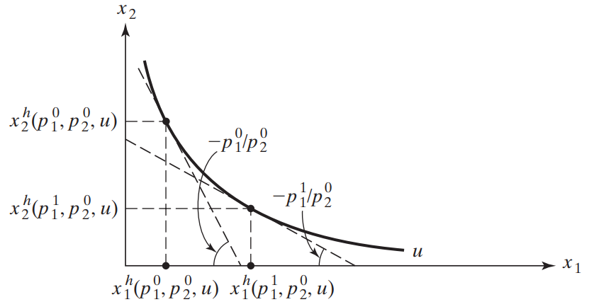
\includegraphics[width=8cm, height=6cm]{pic24}
    \end{center}
  \end{itemize}
  \par
  \underline{Cobb-Douglas Expenditure Function Solution}: for the cobb-douglas equation we have the following minimization problem:
  \begin{gather*}
    \min_{x} \sum_{i=1}^{n}p_{i}x_{i} \ \text{s.t.} \ u(x) \geq \overline{u}
  \end{gather*}
  Using bang-for-buck, from our indirect utility problem, and utility equalization we have two conditions:
  \begin{gather*}
    x_{i} = \frac{\alpha_{i}}{\alpha_{1}}\frac{p_{1}}{p_{i}}x_{1} \ \tag{1} \\
    \prod_{i=1}^{n}x_{i}^{\alpha_{i}} = \overline{u} \ \tag{2}
  \end{gather*}
  Substituting equation $(1)$ into equation $(2)$ we have:
  \begin{align*}
    \overline{u} &= \prod_{i=1}^{n}(\frac{\alpha_{i}}{\alpha_{1}}\frac{p_{1}}{p_{i}}x_{1})^{\alpha_{i}} \\
    \overline{u} &= \prod_{i=1}^{n}(\frac{\alpha_{i}}{\alpha_{1}}\frac{p_{1}}{p_{i}})^{\alpha_{i}} \prod_{i=1}^{n}(x_{1})^{\alpha_{i}} \\
    \overline{u} &= \prod_{i=1}^{n}(\frac{\alpha_{i}}{\alpha_{1}}\frac{p_{1}}{p_{i}})^{\alpha_{i}}x_{1} \ \tag{*}
  \end{align*}
  Note that $\prod_{i=1}^{n}(x_{1})^{\alpha_{i}} = x_{1}$ since the sum of $\alpha_{i}$ is 1 and $x_{i}$ is a constant. Also note that $(*)$ is often referred to as a Hicksian (compensated) Demand function since it can be used to analyze compensated variation and is written as:
  \begin{gather*}
    x_{1}(p,\overline{u}) = \overline{u} \prod_{i=1}^{n} (\frac{\alpha_{1}}{\alpha_{i}}\frac{p_{i}}{p_{1}})^{\alpha_{i}} \ \tag{**}
  \end{gather*}
  In this case our expenditure minimization function is the sum of all goods in the form of equation $(**)$:
  \begin{gather*}
    e(p,\overline{u}) = p_{1}x_{1}(p,\overline{u}) + p_{2}x_{2}(p,\overline{u}) + \dots + p_{n}x_{n}(p,\overline{u}) \ \tag{***}
  \end{gather*}
\subsubsection{Dual Problem}
A solution to the utility maximization problem also solves the expenditure minimization problem (and vice versa), the two problems are in essence a different way of stating the same thing \par \vspace{0.3em}
  \underline{Utility Maximization Problem (u-max)}: find $x(p, I)$ that maximizes $u(x)$ subject to the budget $(p, I)$, i.e. indirect utility
  \par
  \underline{Expenditure Minimization Problem (e-min)}: find $x(p, \overline{u})$ to minimize the expenditure $e(p,\overline{u}) = \sum_{i=1}^{n}p_{i}x_{i}$ incurred to obtain utility $\overline{u}$
  \par
  \underline{Conversion from u-max to e-min}: if a bundle $x$ solves u-max given budget $(p, I)$, then $x$ also solves e-min of obtaining $\overline{u} = u(x)$ given the same prices. In this case we substitute $I$ with $e(p,u)$ in the indirect utility function and solve for $e(p,u)$ to give us the expenditure minimization function
  \begin{itemize}
    \item  \underline{Note}: for notation we can replace $v(p,u)$ with $u$
  \end{itemize}
  \par
  \underline{Conversion from e-min to u-max}: if a bundle $x$ solves the e-min given $(p, \overline{u})$, then $x$ also solves the u-max given budget $(p, \sum_{i=1}^{n}p_{i}x_{i})$, where the income is the cost of the bundle $x$. In this case we substitute $e(p,u)$ with $I$ in the expenditure function and solve for the indirect utility function (i.e. $u = v(p,u)$)
  \begin{itemize}
    \item  \underline{Note}: for notation we can replace $u$ with $v(p,u)$
  \end{itemize}
  \par
  \underline{Cobb-Douglas Expenditure Function from Indirect Utility}: from our previous solution for cobb-douglas indirect utility, we have that
  \begin{gather*}
    u = e(p,u) \prod_{i=1}^{n} (\frac{\alpha_{i}}{p_{i}})^{\alpha_{i}}
  \end{gather*}
  Rearranging for $e(p,u)$ we have:
  \begin{gather*}
    e(p,u) = u \prod_{i=1}^{n} (\frac{p_{i}}{\alpha_{i}})^{\alpha_{i}}
  \end{gather*}
  where the expenditure function is just the inverse of the utility function \begingroup\color{magenta} why is this different to our direct solution for the expenditure function? \endgroup
  \par
\vspace{6mm}
\subsubsection{Welfare}
Welfare refers to consumer surplus, typically the \textit{area under the demand curve minus what the consumer pays}. The change in welfare therefore is the change in consumper surplus, typically the \textit{change in the area under the demand curve minus what the consumer pays} \par \vspace{0.3em}
  \underline{Assumptions}: utility is quasi-linear
  \par
  \underline{Basis}: in general, welfare is based on the question of \textit{how much are you willing to pay to change from situation A to situation B?}
  \par
  \underline{Example 1}: we want to focus on the change in the price of good 1 and its effect on consumer welfare given that $u(x_{1}, x_{2}) = \ln(x_{1}) + x_{2}$
  \begin{itemize}
    \item \underline{Part 1}: we first find demand for goods 1 and 2 as a function of $p_{1}, p_{2}, I > 0$. From this we get:
    \begin{gather*}
      x_{1} =
      \begin{cases}
         & \tfrac{p_{2}}{p_{1}} \text{ if } I \geq p_{2} \\
         & \tfrac{I}{p_{1}} \text{ if } I <  p_{2}
      \end{cases}
    \end{gather*}
    \begin{gather*}
      x_{2} =
      \begin{cases}
         & \tfrac{I}{p_{2}} - 1 \text{ if } I \geq p_{2} \\
         & 0 \text{ if } I < p_{2}
       \end{cases}
    \end{gather*}
    Notice that if income is high enough, your demand for the first good will not depend on income. Thus, we regard quasi-linear utility functions as representing a situation where the good in question (good 1) does not have income effects
    \item  \underline{Part 2}: we want to fix income $I$ and $p_{2}$ as the demand curve is defined only for the price of the good in question, with all other things fixed we can focus on welfare changes from the price of good 1. Setting $I = 80$ and $p_{2} = 40$ means that as $I \geq P_{2}$ we have that $x_{1} = \tfrac{40}{p_{1}}$ and $x_{2} = 1$.
    \\
    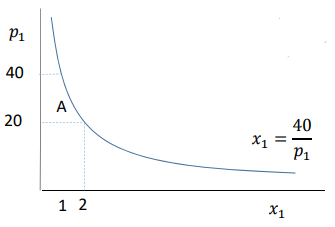
\includegraphics[width=6cm, height=4cm]{pic22}
    \\
    In this case, the area $A$ on the above figure represents the change in consumer surplus (CS) for a price drop from $p_{1} = 40$ to $p_{1}' = 20$. This equals
    \begin{gather*}
      \Delta CS = \int_{20}^{40} \frac{40}{p_{1}} \ dp_{1} = 40[\ln(40) - \ln(20)] = 40 \ln(2) = 27.73
    \end{gather*}
    \item  \underline{Part 3}: Note that at the high price of $p_{1} = 40$, $p_{2} = 40$, and $I = 80$, the optimal bundle is $(x_{1}, x_{2}) = (1, 1)$. When the price drops to $p_{1}' = 20$, the optimal bundle changes to $(x_{1}', x_{2}') = (2, 1)$. We must now examine \textit{how much are you willing to pay at the new prices to have the price drop} by considering how much income we can take away at the new prices($p_{1}'$) to leave the consumer at the same level of utility as before the price change($p_{1}$). \\
    Note that demand for the first good does not depend on income (no income effects), we can take money away from the consumer at the new prices without changing their demand for good 1. At the old prices utility was $u(1,1) = \ln(1) + 1 = 1$. At the new prices, if we take away $m$ from income, then demand for good 1 will remain at $x_{1}' = 2$ and demand for good 2 will drop to:
    \begin{gather*}
      x_{2}' = \frac{80 - m}{40} - 1 = 1 - \frac{m}{40}
    \end{gather*}
    Therefore, utility after we take away $m$ from income will be $u' = \ln(2) + 1 - \tfrac{m}{40}$. We want to know when the utilities from the price drop scenario and the income drop scenario are equal, that is the $m$ that solves $\ln(2) + 1 - \tfrac{m}{40} = 1$. This gives us the change in consumer surplus as:
    \begin{gather*}
      m = 40 \ln(2) = \Delta CS
    \end{gather*}
  \end{itemize}
  \par
\vspace{6mm}
\subsubsection{Compensating Variation (CV)}
Example 1 of the welfare subsection is a demonstration of the \textit{compensating variation} method of computing a welfare change. The compensating variation resulting from a change from $(p, I)$ to $(p', I')$ measures \textit{how much the consumer is willing to pay} to move from $(p, I)$ to $(p', I')$ \par \vspace{0.3em}
  \underline{Measurement of CV}: we can measure CV using the new expenditure function calibrated to the old utility such that $CV = e(p', u) - I'$, where $u$ is the utility obtained at the initial solution $(p, I)$. Alternatively, we can write this as:
  \begin{gather*}
    CV = e(p',u') - e(p',u) = I' - e(p',u)
  \end{gather*}
  \par
  \underline{Translation}: CV measures how much income can be taken away from the person in the new situation, to make that person just as well off as in the initial situation
  \begin{itemize}
    \item  \underline{Note}: CV will be negative when the new situation makes the person worse off
  \end{itemize}
  \par
  \underline{Difference between CV and $\Delta$CS}: the use of CV is regarded as the correct measure of welfare change, since if income effects are not small then the change in consumer surplus will over or under state welfare changes. However in the case where income effects are negligible (i.e. when we have quasi-linear $u$) then the change in consumer surplus can be used instead.
  \begin{itemize}
    \item  \underline{Note}: the change in consumer surplus is based on the idea that how much you pay for the first few units does not affect your marginal willingness to pay for additional units \begingroup\color{magenta} how? \endgroup. If this is not true, then the change in CS will be biased
  \end{itemize}
  \par
\vspace{6mm}
\subsubsection{Exercise 1}
Consider the utility function $u(x,y) = xy$ for Cameron. Suppose that initially $I = 100$, $p_{x} = 1$, and $p_{y} = 4$ \par \vspace{0.3em}
\begin{itemize}
  \item  \underline{Question 1}: find the indirect utility function and expenditure minimization function for Cameron and  the respective values for each
  \begin{itemize}
    \item  \underline{Answer}: from the bang-for-buck and budget set conditions we have:
    \begin{gather*}
      \frac{y}{p_{x}} = \frac{x}{p_{y}} \ \tag{1} \\
      p_{x}x + p_{y}y = I \ \tag{2}
    \end{gather*}
    Rearranging equation $(1)$ we can solve for $y$:
    \begin{gather*}
      y = x \frac{p_{x}}{p_{y}} \ \tag{*}
    \end{gather*}
    Substituting $(*)$ into equation $(2)$ yields:
    \begin{align*}
      p_{x}x + xp_{x} &= I \\
      \therefore x &= \frac{I}{2p_{x}} \ \tag{**}
    \end{align*}
    Likewise, rearranging equation $(1)$ to solve for $x$ and substituting this into $(2)$ yields:
    \begin{gather*}
      y = \frac{I}{2p_{y}} \ \tag{***}
    \end{gather*}
    Equations $(**)$ and $(***)$ give us optimal quantities of $x$ and $y$ for our known parameters so we can use them to solve for indirect utility:
    \begin{align*}
      v(p,I) &= \max u(x,y) | p_{x}x + p_{y}y = I \\
      v(p,I) &= \frac{I}{2p_{x}} \cdot \frac{I}{2p_{y}} \\
      v(p,I) &= \frac{I^{2}}{4p_{x}p_{y}} \ \tag{$\star$}
    \end{align*}
    In this case $(\star)$ can be stated as a expenditure function where:
    \begin{align*}
      v(p,I) &= \frac{e(p,v(p,I))^{2}}{4p_{x}p_{y}} \\
      e(p,v(p,I)) &= 2 \sqrt{v(p,I)p_{x}p_{y}} \ \tag{$\star \star$}
    \end{align*}
    For $p_{x} = 1$, $p_{y} = 4$, and $I = 100$, we have from $(\star)$ that:
    \begin{gather*}
      v(p,I) = \frac{100^{2}}{4 \cdot 1 \cdot 4} = 625
    \end{gather*}
    Using the value of $v(p,I)$ in equation $(\star \star)$ we have:
    \begin{gather*}
      e(p,v(p,I)) = 2 \sqrt{625 \cdot 1 \cdot 4} = 100
    \end{gather*}
  \end{itemize}
  \item  \underline{Question 2}: suppose there is an economic downturn that lowers the price of $y$ and poor Cameron's income. Calculate the Compensating Variation (CV) when the price of good $y$ falls to $p_{y}' = 2$ and income falls to $I' = 50$
  \begin{itemize}
    \item  \underline{Answer}: to measure CV we use the formula
    \begin{gather*}
      CV = I' - e(p', u)
    \end{gather*}
    Using new prices, $p_{x}' = 1$ and $p_{y}' = 2$, as well as $u$ given by $v(p,I) = 625$ prior to the change, we have
    \begin{gather*}
      e(p',u) = 2 \sqrt{625 \cdot 1 \cdot 2} = 70.71
    \end{gather*}
    Therefore, since $I' = 50$ we have
    \begin{gather*}
      CV = 50 - 70.71 = -20.71
    \end{gather*}
    meaning that Cameron is willing to pay $-20.71$, or equivalently needs to be compensated $20.71$, for the change
  \end{itemize}
  \item  \underline{Question 3}: suppose now that Cameron is the lucky child of a lecturer, so he keeps his income of 100 even in the downturn and only experiences the price fall in good $y$
  \begin{itemize}
    \item  \underline{Answer}: with prices $p_{x}' = 1$, $p_{y}' = 2$, and $I' = 100$ we have:
    \begin{gather*}
      CV = 100 - 70.71 = 29.29
    \end{gather*}
    meaning that Cameron is willing to pay $29.29$, or equivalently will compensate others $29.29$, for the change
  \end{itemize}
  \item  \underline{Question 4}: re-calculate the consumer surplus (CS) change due to the price drop mentioned in question 3 using the area under Cameron's demand curve for good $y$. How much is the difference between CS and CV? Does CS over or under estimate the CV? Can you explain the reason for the over or under estimation in terms of income effects
  \begin{itemize}
    \item  \underline{Answer}: since only the price of good y changes, the change in consumer surplus is just the change under the demand curve for good y:
    \begin{align*}
      \Delta CS &= \int_{2}^{4} \frac{I}{2p_{y}} \ d p_{y} \\
      &= \int_{2}^{4} \frac{50}{p_{y}} \ d p_{y} \\
      &= 50 \ln(4) - 50 \ln(2) \\
      \Delta CS &= 34.66
    \end{align*}
    This is a significant overestimate of compensating variation due to ignoring income effects
  \end{itemize}
\end{itemize}
\par
\vspace{6mm}
\subsubsection{Exercise 2}
The Stone-Geary utility function has the form
\begin{gather*}
  u(x) = \prod_{i=1}^{n}(x_{i} - a_{i})^{b_{i}}
\end{gather*}
where $b_{i} > 0$ and $\sum_{i=1}^{n}b_{i} = 1$. The $a_{i} \geq 0$ are often interpreted as subsistence levels for the goods and to ensure that the utility function is real value we restrict $x_{i} \geq a_{i}$. Therefore, income $I$ is at least $\sum_{i=1}^{n} p_{i}a_{i}$ \par \vspace{0.3em}
\begin{itemize}
  \item  \underline{Question 1}: derive the indirect utility function and the expenditure function
  \begin{itemize}
    \item  \underline{Answer}: we have the following bang-for-buck conditions in terms of good 1:
    \begin{gather*}
      \frac{b_{1}(x_{1}-a_{1})^{b_{1}-1}\prod_{i \neq 1}^{n}(x_{i} - a_{i})^{b^{1}}}{p_{1}} = \frac{b_{j}(x_{j} - a_{j})^{b_{j}-1} \prod_{i \neq j}^{n}(x_{i} - a_{i})^{b_{i}}}{p_{j}} \ \tag{1}
    \end{gather*}
    We can expand out the summations from equation $(1)$ as follows:
    \begin{gather*}
      \frac{b_{1}(x_{1}-a_{1})^{b_{1}-1} (x_{j} - a_{j})^{b_{j}} \prod_{i \neq 1,j}^{n}(x_{i} - a_{i})^{b^{1}}}{p_{1}} = \frac{b_{j}(x_{j} - a_{j})^{b_{j}-1} (x_{1} - a_{1})^{b_{1}} \prod_{i \neq j,1}^{n}(x_{i} - a_{i})^{b_{i}}}{p_{j}}
    \end{gather*}
    We can cancel out these summations to yield:
    \begin{align*}
      \frac{b_{1}(x_{1}-a_{1})^{b_{1}-1} (x_{j} - a_{j})^{b_{j}}}{p_{1}} &= \frac{b_{j}(x_{j} - a_{j})^{b_{j}-1} (x_{1} - a_{1})^{b_{1}}}{p_{j}} \\
      b_{1}(x_{1} - a_{1})^{-1} \frac{p_{j}}{p_{1}} &= b_{j}(x_{j} - a_{j})^{-1}
    \end{align*}
    We can rearrange this for $x_{j}$ as a function of $x_{1}$:
    \begin{align*}
      (x_{j} - a_{j})^{-1} &= \frac{b_{1}}{b_{j}} \frac{p_{j}}{p_{1}} (x_{1} - a_{1})^{-1} \\
      x_{j}^{-1} &= \frac{b_{1}}{b_{j}} \frac{p_{j}}{p_{1}} (x_{1} - a_{1})^{-1} + a_{j}^{-1} \\
      \therefore x_{j} &= \frac{b_{j}}{b_{1}}\frac{p_{1}}{p_{j}} (x_{1} - a_{1}) + a_{j} \ \tag{*}
    \end{align*}
    Inserting $(*)$ into our budget constraint and noting that $\sum_{i=1}^{n} b_{j} = 1$ yields $x_{j}$ as a function of known parameters:
    \begin{align*}
      I &= \sum_{j=1}^{n} p_{j}x_{j} \\
      &= \sum_{j=1}^{n} p_{j}\big( \frac{b_{j}}{b_{1}}\frac{p_{1}}{p_{j}} (x_{1} - a_{1}) + a_{j} \big) \\
      &= \sum_{j=1}^{n} \frac{b_{j}}{b_{1}} p_{1}(x_{1} - a_{1}) + \sum_{j=1}^{n} p_{j} a_{j} \\
      I &= \frac{p_{1}(x_{1} - a_{1})}{b_{1}} + \sum_{j=1}^{n} p_{j}a_{j} \\
      I b_{1} &= p_{1}x_{1} - p_{1}a_{1} + b_{1} \sum_{j=1}^{n} p_{j}a_{j} \\
      x_{1} &= \frac{b_{1}(I - \sum_{j=1}^{n}p_{j}a_{j})}{p_{1}} + a_{1} \ \tag{**}
    \end{align*}
    Inserting equation $(**)$ into equation $(*)$ yields:
    \begin{align*}
      x_{j} &= \frac{b_{j}}{b_{1}} \frac{p_{1}}{p_{j}} (\frac{b_{1}(I - \sum_{j=1}^{n}p_{j}a_{j})}{p_{1}} + a_{1} - a_{1}) + a_{j} \\
      x_{j} &= \frac{b_{j}}{p_{j}}(I - \sum_{j=1}^{n}p_{j}a_{j}) + a_{j} \ \tag{***}
    \end{align*}
    Substituting equation $(***)$ into our utility function gives us the indirect utility function:
    \begin{gather*}
      v(p,I) = \prod_{j=1}^{n} \big[ \frac{b_{j}}{p_{j}}(I - \sum_{j=1}^{n}p_{j}a_{j}) \big]^{b_{j}}
    \end{gather*}
    Note that since $(I - \sum_{j=1}^{n}p_{j}a_{j})$ is a constant with respect to the product $\prod_{j=1}^{n}$, we have:
    \begin{gather*}
      v(p,I) = (I - \sum_{j=1}^{n}p_{j}a_{j}) \prod_{j=1}^{n} (\frac{b_{j}}{p_{j}})^{b_{j}} \ \tag{$\star$}
    \end{gather*}
    To transform $(\star)$ into an expenditure minimization function we substitute $I$ for $e(p,v(p,I))$ and rearrange as follows:
    \begin{align*}
      v(p,I) &= (e(p,v(p,I)) - \sum_{j=1}^{n}p_{j}a_{j}) \prod_{j=1}^{n} (\frac{b_{j}}{p_{j}})^{b_{j}} \\
      e(p,v(p,I)) &= \frac{v(p,I)}{\prod_{j=1}^{n} (\frac{b_{j}}{p_{j}})^{b_{j}}} + \sum_{j=1}^{n}p_{j}a_{j} \\
      e(p,v(p,I)) &= =v(p,I) \prod_{j=1}^{n} (\frac{p_{j}}{b_{j}})^{b_{j}} + \sum_{j=1}^{n}p_{j}a_{j} \ \tag{$\star \star$}
    \end{align*}
  \end{itemize}
  \item  \underline{Question 2}: show that $b_{i}$ measures the share of discretionary income that is spent on good $i$ in excess of what $a_{i}$ costs, where discretionary income is defined as $I - \sum_{i=1}^{n}p_{i}a_{i}$. Note that the term discretionary income is used since this is the income above what is needed to ensure that $x_{i} \geq a_{i}$
  \begin{itemize}
    \item  \underline{Answer}: from equation $(***)$ we can solve for $b_{j}$ as:
    \begin{gather*}
      b_{j} = \frac{p_{j}(x_{j}-a_{j})}{(I - \sum_{j=1}^{n}p_{j}a_{j})}
    \end{gather*}
    Note that the numerator in this case is the amount spent on good j above the subsistence amount of good j required, since $a_{j}$ is the subsistence amount needed and $x_{j}$ is the total amount consumed. The denominator is the discretionary income remaining after consuming the substitence amounts of all goods. Therefore, $b_{j}$ measures the amount spent to consume the non-subsistence number of good j as a share of non-subsistence income, i.e. the share of discretionary income spent on good j
  \end{itemize}
\end{itemize}
\par
\vspace{6mm}
\subsubsection{Exercise 3}
Consider the utility function $u(x_{1}, x_{2}) = \ln x_{1} + x_{2}$ where $x_{1} > 0$ so that utility is not only real-valued but also well-defined \par \vspace{0.3em}
\begin{itemize}
  \item  \underline{Question 1}: find the demand functions, called Hicksian demand functions, which come from the expenditure minimization problem
  \begin{itemize}
    \item  \underline{Answer}: our expenditure minimization problem is:
    \begin{gather*}
      \min_{x_{1},x_{2}} \ p_{1}x_{1} + p_{2}x_{2} \\
      \text{s.t.} \ \ u(x_{1}, x_{2}) \geq \overline{u}
    \end{gather*}
    We need to first solve for $x_{1}$ using our bang-for-back condition:
    \begin{align*}
      \frac{\tfrac{\partial u}{\partial x_{1}}}{p_{1}} &= \frac{\tfrac{\partial u}{\partial x_{2}}}{p_{2}} \\
      \frac{\tfrac{1}{x_{1}}}{p_{1}} &= \frac{1}{p_{2}} \\
      \therefore x_{1} &= \frac{p_{2}}{p_{1}}
    \end{align*}
    From the $x_{1}$ in the above equation and our expenditure function, we have the following 2 conditions:
    \begin{gather*}
      x_{1} = \frac{p_{2}}{p_{1}} \ \tag{1} \\
      \ln x_{1} + x_{1} = \overline{u} \ \tag{2}
    \end{gather*}
    Substituting equation $(2)$ into $(1)$ yields:
    \begin{gather*}
      \ln (\frac{p_{2}}{p_{1}}) + x_{1} = \overline{u}
    \end{gather*}
    Note that due to the relatively huge but diminishing returns of low levels of $x_{1}$, we will either spend all income on $x_{1}$ (if $u \leq \ln (\frac{p_{2}}{p_{1}})$) or spend income on both $x_{1}$ and $x_{2}$ (if $u > \ln (\frac{p_{2}}{p_{1}})$). \\
    If we are spending all income on $x_{1}$ then we have that $\ln(x_{1}) = \overline{u}$ and therefore:
    \begin{align*}
      x_{1} &= \exp (\overline{u}) \ \tag{*} \\
      x_{2} &= 0 \ \tag{**}
    \end{align*}
    Of we are spending income on both $x_{1}$ and $x_{2}$ then we have that:
    \begin{align*}
      x_{1} &= \frac{p_{2}}{p_{1}} \ \tag{***} \\
      x_{2} &= u - \ln (\frac{p_{2}}{p_{1}}) \ \tag{****}
    \end{align*}
    Combining equations (*), (**), (***), and (****) gives us our Hicksian demand function:
    \begin{align*}
      x_{1}(p,\overline{u}) &=
      \begin{cases}
         \exp(\overline{u}) & \text{ if } u \leq \ln (\frac{p_{2}}{p_{1}}) \\
         \frac{p_{2}}{p_{1}} & \text{ if } u > \ln (\frac{p_{2}}{p_{1}})
       \end{cases} \ \tag{3}
      \\
      x_{2}(p, \overline{u}) &=
      \begin{cases}
         0 & \text{ if } u \leq \ln (\frac{p_{2}}{p_{1}}) \\
         u - \ln (\frac{p_{2}}{p_{1}}) & \text{ if } u > \ln (\frac{p_{2}}{p_{1}})
       \end{cases} \ \tag{4}
    \end{align*}
    Note that our expenditure function is just the sum of all goods (at optimal consumption) multiplied by their price:
    \begin{gather*}
      e(p,u) = x_{1}(p,\overline{u})p_{1} + x_{2}(p,\overline{u})p_{2}
    \end{gather*}
    Therefore, from out hicksian demand equations (3) and (4) we have:
    \begin{gather*}
      e(p,u) =
      \begin{cases}
        p_{1} \exp(u) & \text{ if } u \leq  \ln (\frac{p_{2}}{p_{1}}) \\
        p_{2}(1+u- \ln (\frac{p_{2}}{p_{1}})) & \text{ if } u >  \ln (\frac{p_{2}}{p_{1}})
      \end{cases} \ \tag{$\star$}
    \end{gather*}
  \end{itemize}
  \item  \underline{Question 2}: use the expenditure function to find the indirect utility function
  \begin{itemize}
    \item  \underline{Answer}: we can find indirect utility by setting $u = v(p, e(p,u))$ and rearranging for $v(p, e(p,u))$ in equation $(\star)$. \\ For the $u \leq \ln (\tfrac{p_{2}}{p_{1}})$ case we have:
    \begin{align*}
      e(p,u) = p_{1}\exp (v(p,e(p,u))) \\
      \therefore v(p,e(p,u)) = \ln (\frac{e(p,u)}{p_{1}})
    \end{align*}
    which occurs when $\ln(\tfrac{I}{p_{1}}) \leq \ln (\tfrac{p_{2}}{p_{1}}) \equiv \ln(I) \leq \ln(p_{2})$. \\ For the $u > \ln (\tfrac{p_{2}}{p_{1}})$ we have:
    \begin{align*}
      e(p,u) &= p_{2}(1 + v(p,u) - \ln (\frac{p_{2}}{p_{1}})) \\
      v(p,u) &= \frac{e(p,u)}{p_{2}} + \ln \ln (\frac{p_{2}}{p_{1}}) - 1
    \end{align*}
    which occurs when $\ln (I) > \ln (p_{2})$
  \end{itemize}
\end{itemize}
\par
\vspace{6mm}
\subsubsection{Exercise 3}
Consider the following demand system:
\begin{gather*}
  x(p,I) = \frac{Ip_{z}}{4p_{x}p_{y}}; \ y(p,I) = \frac{I}{4p_{y}}; \ z(p,I) = 0
\end{gather*}
\par \vspace{0.3em}
\begin{itemize}
  \item  \underline{Question 1}: is each demand function homogeneous of degree zero in prices and income
  \begin{itemize}
    \item  \underline{Answer}: equation $x(p,I)$ is homogeneous of degree zero since if we multiply $I$ and $p$ by some constant $t$ we have:
    \begin{gather*}
        t^{k}x(p,I) = \frac{(tI)(tp_{z})}{4(tp_{x})(tp_{y})} = \frac{t^{2}Ip_{z}}{4t^{2}p_{x}p_{y}} = \frac{Ip_{z}}{4p_{x}p_{y}}
    \end{gather*}
    where $k$ must equal 0. Similarly $y(p,I)$ is homogeneous of degree zero since we have:
    \begin{gather*}
      t^{0}y(p,I) = \frac{tI}{4tp_{y}} = \frac{I}{4p_{y}}
    \end{gather*}
    $z(p,I)$ is also homogeneous of degree zero since its demand is not affected by any inputs.
  \end{itemize}
  \item  \underline{Question 2}: argue that this demand system does not satisfy budget exhaustion
  \begin{itemize}
    \item  \underline{Answer}: budget exhaustion occurs when the utility function causes consumption to be such that
    \begin{gather*}
      \textbf{p}\textbf{x} = \textbf{I}
    \end{gather*}
    In this case we have that for budget exhaustion to occur:
    \begin{gather*}
      p_{x}x + p_{y}y + p_{z}z = I \ \tag{1}
    \end{gather*}
    Substituting the given optimal demand system into equation $(1)$, we have that:
    \begin{align*}
      p_{x}(\frac{Ip_{z}}{4p_{x}p_{y}}) + p_{y}(\frac{I}{4p_{y}}) + p_{z} \cdot 0 &= I
      \therefore \frac{Ip_{z}}{4p_{y}} + \frac{I}{4} &= I \ \tag{2}
    \end{align*}
    Note that from equation $(2)$ we have that budget exhaustion does not hold if $\tfrac{p_{z}}{p_{y}} \ngeq 3$ since:
    \begin{align*}
      I(\frac{p_{z}}{4p_{y}} + \frac{1}{4}) &= I \\
      \frac{p_{z}}{4p_{y}} + \frac{1}{4} &= 1 \\
      \frac{p_{z}}{p_{y}} &= 3
    \end{align*}
  \end{itemize}
  \item  \underline{Question 3}: keeping $x(p,I)$ and $y(p,I)$ as defined above, if budget exhaustion is required then what must $z(p,I)$ be
  \begin{itemize}
    \item  \underline{Answer}: to find $z(p,I)$ such that budget exhaustion holds, we substitute all demand functions except for $z$'s into budget the constraint given by equation (1):
    \begin{align*}
      p_{x}(\frac{Ip_{z}}{4p_{x}p_{y}}) + p_{y}(\frac{I}{4p_{y}}) + p_{z}z &= I \\
      \therefore \frac{Ip_{z}}{4p_{y}} + \frac{I}{4} + p_{z}z &= I
    \end{align*}
    We then rearrange this equation to solve for $z(p,I)$:
    \begin{align*}
      p_{z}z &= I - \frac{Ip_{z}}{4p_{y}} - \frac{I}{4} \\
      z &= \frac{I}{p_{z}} - \frac{I}{4p_{y}} - \frac{I}{4p_{z}} \\
      \therefore z(p,I) &= I(\frac{0.75}{p_{z}} - \frac{0.25}{p_{y}})
    \end{align*}
  \end{itemize}
  \item  \underline{Question 4}: is the new demand for each good homogeneous of degree zero in prices and income
  \begin{itemize}
    \item  \underline{Answer}: $z(p,I)$ is homogeneous of degree 0 since:
    \begin{gather*}
      t^{k}z(p,I) = tI (\frac{0.75}{tp_{z}} - \frac{0.25}{tp_{y}}) = I (\frac{0.75}{p_{z}} - \frac{0.25}{p_{y}})
    \end{gather*}
    where $k$ must equal 0. Therefore, using the results from question 2 we have that all 3 demand functions are homogeneous of degree zero
  \end{itemize}
  \item  \underline{Question 5}: what does your answer to question 4 suggest about the likelihood that this demand system is obtained from utility maximization subject to the budget constraint
  \begin{itemize}
    \item  \underline{Answer}: question 4 gives no evidence to suggest otherwise as utility maximization subject to the budget constraint will generate demands that are homogeneous of degree zero in prices and income and these demands have this property
  \end{itemize}
\end{itemize}
\par
\vspace{6mm}
\subsubsection{Exercise 4}
Let $u(x) = \sqrt{x_{1}x_{2}} + \sqrt{x_{3}}$
\par \vspace{0.3em}
\begin{itemize}
  \item  \underline{Question 1}: are the preferences convex
  \begin{itemize}
    \item  \underline{Answer}: preferences are convex if and only if for all $x,y \in R^{+}$ if $x \succeq y$ then for all $t \in [0,1]$: $tx + (1-t)y \succeq y$ \\ This means that if indifference curves are convex then we have convex preferences. To construct an indifference curve for this function, suppose that $u(x) = 15$ and $x_{1} = x_{2}$. This results in the following relationship:
    \begin{align*}
      u(x) &= \sqrt{x_{1}x_{2}} + \sqrt{x_{3}} \\
      15 &= x_{1} + \sqrt{x_{3}} \\
      \therefore x_{2} = x_{1} &= 15 - \sqrt{x_{3}} \ \tag{*}
    \end{align*}
    Note that the indifference curve representing $u(x) = 15$, in the case where $x_{1} = x_{2}$, given by equation $(*)$ is convex. This can be seen in the below graph where the better than set, $G(X)$, is a convex set \\
    \begin{center}
      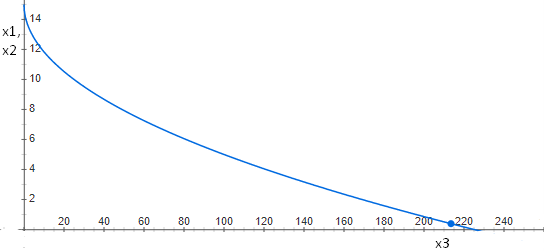
\includegraphics[width=6cm, height=4cm]{pic26}
    \end{center}
    \begin{itemize}
      \item  \underline{Note}: if convexity did not hold we could use equation $(*)$ to construct 2 bundles and test their relationship to an in between 3rd bundle
    \end{itemize}
    \item  \underline{Alternate Answer}: since $\sqrt{x_{1}x_{2}}$ and $\sqrt{x_{3}}$ are both concave functions and the sum of concave functions is concave, it follows that $u(x)$ is concave. Since every concave function is quasi-concave, it follows that $u(x)$ is quasi-concave. Since quasi-concavity of the utility function is equivalent to convexity of the preferences it represents, the preferences are convex
  \end{itemize}
  \item  \underline{Question 2}: concentrating on situtations where $I > \tfrac{p_{1}p_{2}}{p_{3}}$, verify that the demand functions are
  \begin{gather*}
    x_{1}(p,I) = \frac{1}{2p_{1}}(I - \frac{p_{1}p_{2}}{p_{3}}); \ x_{2}(p,I) = \frac{1}{2p_{2}}(I - \frac{p_{1}p_{2}}{p_{3}}); \ x_{3}(p,I) = \frac{p_{1}p_{2}}{p_{3}^{2}}
  \end{gather*}
  \begin{itemize}
    \item  \underline{Answer}: we have the following bang-for-buck conditions:
    \begin{gather*}
      \frac{\tfrac{\partial u}{\partial x_{1}}}{p_{1}} = \frac{\tfrac{\partial u}{\partial x_{2}}}{p_{2}} = \frac{\tfrac{\partial u}{\partial x_{3}}}{p_{3}} \\
      \frac{0.5x_{1}^{-0.5}x_{2}^{0.5}}{p_{1}} = \frac{0.5x_{1}^{0.5}x_{2}^{-0.5}}{p_{2}} = \frac{0.5x_{3}^{-0.5}}{p_{3}} \ \tag{1}
    \end{gather*}
    Condition $(1)$ yields the following relationships when comparing the bang-for-buck for goods 1 and 2:
    \begin{align*}
      \frac{0.5x_{1}^{-0.5}x_{2}^{0.5}}{p_{1}} &= \frac{0.5x_{1}^{0.5}x_{2}^{-0.5}}{p_{2}} \\
      x_{1}^{-1} &= (\frac{p_{1}}{p_{2}})x_{2}^{-1} \\
      \therefore x_{1} &= (\frac{p_{2}}{p_{1}})x_{2} \ \tag{2} \\
      \therefore x_{2} &= (\frac{p_{1}}{p_{2}})x_{1} \ \tag{3}
    \end{align*}
    Condition $(1)$ also yields the following relationship when comparing goods 2 and 3:
    \begin{align*}
      \frac{0.5x_{1}^{0.5}x_{2}^{-0.5}}{p_{2}} &= \frac{0.5x_{3}^{-0.5}}{p_{3}} \\
      x_{3}^{-0.5} &= x_{1}^{0.5}x_{2}^{-0.5} (\frac{p_{3}}{p_{2}}) \\
      x_{3} = x_{1}^{-1}x_{2} (\frac{p_{3}}{p_{2}})^{-2} \\
      \therefore x_{3} = \frac{x_{2}}{x_{1}} (\frac{p_{2}}{p_{3}})^{2} \ \tag{4}
    \end{align*}
    By substituting equation $(3)$ into equation $(4)$ we get our marshallian demand for $x_{3}$:
    \begin{align*}
      x_{3} &= \frac{x_{1}(\tfrac{p_{1}}{p_{2}})}{x_{1}} (\frac{p_{2}}{p_{3}})^{2} \\
      x_{3} &= (\frac{p_{1}}{p_{2}})(\frac{p_{2}}{p_{3}})^{2} \\
      \therefore x_{3}(p,I) &= \frac{p_{1}p_{2}}{p_{3}^{2}} \ \tag{5}
    \end{align*}
    Inserting equations $(2)$, $(3)$, and $(5)$ into our budget constraint yields:
    \begin{align*}
      p_{1}x_{1} + p_{2}x_{2} + p_{3}x_{3} &= I  \\
      p_{1(\frac{p_{2}}{p_{1}})x_{2}}) + p_{2}(\frac{p_{1}}{p_{2}}x_{1}) + p_{3}(\frac{p_{1}p_{2}}{p_{3}^{2}}) &= I \\
      p_{2}x_{2} + p_{1}x_{1} + \frac{p_{1}p_{2}}{p_{3}} &= I \ \tag{6}
    \end{align*}
    Substituting equation $(2)$ into $(6)$ yields our marshallian demand for $x_{2}$:
    \begin{align*}
      p_{2}x_{2} + p_{1}x_{1} + \frac{p_{1}p_{2}}{p_{3}} &= I \\
      2p_{2}x_{2} &= I - \frac{p_{1}p_{2}}{p_{3}} \\
      \therefore x_{2}(p,I) &= \frac{1}{2p_{2}}(I - \frac{p_{1}p_{2}}{p_{3}}) \ \tag{7}
    \end{align*}
    Substituting equation $(3)$ into $(6)$ yields our marshallian demand for $x_{1}$:
    \begin{align*}
      p_{2}x_{2} + p_{1}x_{1} + \frac{p_{1}p_{2}}{p_{3}} &= I \\
      \therefore x_{1}(p,I) &= \frac{1}{2p_{1}}(I - \frac{p_{1}p_{2}}{p_{3}}) \ \tag{8}
    \end{align*}
    Overall, equations $(5)$, $(6)$, and $(7)$ give us the demand functions for $x_{3}$, $x_{2}$, and $x_{1}$, respectively, when $I > \frac{p_{1}p_{2}}{p_{3}}$
  \end{itemize}
  \item  \underline{Question 3}: find the indirect utility function when $I > \tfrac{p_{1}p_{2}}{p_{3}}$
  \begin{itemize}
    \item  \underline{Answer}: to find the indirect utility function we substitute our optimal demand equations $(5)$, $(6)$, and $(7)$ into the utility function as follows:
    \begin{align*}
      u(x) &= \sqrt{x_{1}x_{2}} + \sqrt{x_{3}} \\
      &= \sqrt{\frac{1}{2p_{1}}(I - \frac{p_{1}p_{2}}{p_{3}})\frac{1}{2p_{2}}(I - \frac{p_{1}p_{2}}{p_{3}})} + \sqrt{\frac{p_{1}p_{2}}{p_{3}^{2}}} \\
      &= \sqrt{(I - \frac{p_{1}p_{2}}{p_{3}})^{2}\frac{1}{4p_{1}p_{2}}} + \frac{\sqrt{p_{1}p_{2}}}{\sqrt{p_{3}^{2}}} \\
      &= (I - \frac{p_{1}p_{2}}{p_{3}})0.5 \frac{1}{\sqrt{p_{1}p_{2}}} + \frac{\sqrt{p_{1}p_{2}}}{p_{3}} \\
      &= 0.5I(p_{1}p_{2})^{-0.5} - 0.5 \frac{p_{1}p_{2}(p_{1}p_{2})^{-0.5}}{p_{3}} + \frac{(p_{1}p_{2})^{0.5}}{p_{3}} \\
      \therefore v(p,I) &= 0.5 I(p_{1}p_{2})^{-0.5} + 0.5 \frac{(p_{1}p_{2})^{0.5}}{p_{3}} \ \tag{$\star$}
    \end{align*}
  \end{itemize}
  \item  \underline{Question 4}: calculate the CV for a change in prices and income from $(p,I) = ((2,2,2), 10)$ to $(p',I') = ((4,1,1),20)$
  \begin{itemize}
    \item  \underline{Answer}: we must first solve for the expenditure minimization function by substituting $I$ for $e(p,v(p,I))$ in the indirect utility equation $(\star)$ and rearranging for $e(p,v(p,I))$:
    \begin{align*}
      v(p,I) &= 0.5 e(p,v(p,I))(p_{1}p_{2})^{-0.5} + 0.5 \frac{(p_{1}p_{2})^{0.5}}{p_{3}} \\
      0.5 e(p,v(p,I))(p_{1}p_{2})^{-0.5} &= v(p,I) - 0.5 \frac{(p_{1}p_{2})^{0.5}}{p_{3}} \\
      \therefore e(p,v(p,I)) &= 2v(p,I)(p_{1}p_{2})^{0.5} - \frac{p_{1}p_{2}}{p_{3}} \ \tag{$\star$}
    \end{align*}
    CV can be calculated using the below formula:
    \begin{gather*}
      CV = I' - e(p', u)
    \end{gather*}
    Setting $u = v(p,I)$ we have:
    \begin{align*}
      u &= 0.5 I(p_{1}p_{2})^{-0.5} + 0.5 \frac{(p_{1}p_{2})^{0.5}}{p_{3}} \\
      u &= 0.5 \cdot 10 (2 \cdot 2)^{-0.5} + 0.5 \frac{(2 \cdot 2)^{0.5}}{2} \\
      \therefore u &= 3
    \end{align*}
    From $u=3$ we have that:
    \begin{align*}
      e(p',u &= 2u(p_{1}'p_{2}')^{0.5} - \frac{p_{1}'p_{2}'}{p_{3}'} \\
      &= 2 \cdot 3 (4 \cdot 1)^{0.5} - \frac{4 \cdot 1}{1} \\
      \therefore e(p',u) &= 8
    \end{align*}
    Using that $e(p',u) = 8$ and $I' = 20$, compensating variation is:
    \begin{gather*}
      CV = 20 - 8 = 12
    \end{gather*}
    So you would be willing to pay/compensate others 12 to go from $(p,I)$ to $(p',I')$
  \end{itemize}
  \item  \underline{Question 5}: how does the demand system change if $I < \tfrac{p_{1}p_{2}}{p_{3}}$
  \begin{itemize}
    \item  \underline{Answer}: from equation $(6)$ we have that:
    \begin{align*}
      p_{2}x_{2} + p_{1}x_{1} + \frac{p_{1}p_{2}}{p_{3}} &= I
      p_{2}x_{2} + p_{1}x_{1} &= I - \frac{p_{1}p_{2}}{p_{3}} < 0  \ \text{if} \ I < \frac{p_{1}p_{2}}{p_{3}}
    \end{align*}
    Since $p_{2}x_{2}$ and $p_{1}x_{1}$ cannot be negative, we have that their consumption must be $0$ if $I < \tfrac{p_{1}p_{2}}{p_{3}}$. Therefore all income must be spent on $x_{3}$ and so our demand system becomes:
    \begin{gather*}
      x_{1}(p,I) = 0; \ x_{2}(p,I) = 0; \ x_{3}(p,I) = \frac{I}{p_{3}}, \ \text{if} \  I < \frac{p_{1}p_{2}}{p_{3}}
    \end{gather*}
    Intuitively this makes sense since if $I < \tfrac{p_{1}p_{2}}{p_{3}}$ this means that $p_{1}p_{2}$ is high relative to $p_{3}$ and so consumption is going to be focused on $x_{3}$. In this case, since we have diminishing marginal returns, income will only be spent on $x_{1}x_{2}$ once a given level of $x_{3}$ is consumed (or if $x_{3}$ is relatively expensive) - which occurs only when $I > \frac{p_{1}p_{2}}{p_{3}}$
  \end{itemize}
\end{itemize}

\vspace{2.5mm}
\subsection{Uncertainty}
In this section, the concepts of expected utility theory, the St Petersburg Paradox, and risk are discussed \par
\vspace{6mm}
\subsubsection{Set of Alternatives/Lotteries}
The standard set of alternatives for situations involving uncertainty is a set of lotteries - wherein a single lottery is a probability distribution over some set of outcomes $Z$. Here the set of alternatives is the set of these lotteries and is denoted by $L$ with a single lottery denoted by lower case letters $p, \ q, \ etc$. Preferences $\succeq$ are expressed as a binary relation on the set of lotteries $L$ \par \vspace{0.3em}
  \underline{Outcomes in Z}: $Z$ could include things such as a bundle of goods (i.e. points in $\mathbb{R}_{+}^{n}$), amounts of money (i.e. points in $\mathbb{R}$), or even complete descriptions of a situation. Probable are referred to as certain outcomes within $Z$
  \begin{itemize}
    \item \underline{Note}: the outcomes in Z have certainty in information/value, however there is uncertainty over which outcome is going to occur since we are in a lottery
  \end{itemize}
  \par
\vspace{6mm}
\subsubsection{Subjective Uncertainty}
This occurs when there is uncertainty about the probabilities within a given lottery, with these probabilities interpreted as beliefs. In this case, in addition to the set $Z$ of certain outcomes, there is a state space $S$ (i.e. different states of the world) which assigns different possible probabilities for the lottery \par \vspace{0.3em}
  \underline{Acts}: the function $f: S \rightarrow Z$ is referred to as an act, with preferences defined over the set of acts. This assigns for each state of the world $S$ the corresponding set of certain outcomes $Z$
  \par
\vspace{6mm}
\subsubsection{St Petersburg Paradox}
You face a situation where you can select either:
\begin{itemize}
  \item  \underline{Option A}: take \$ 1000 for certain
  \item  \underline{Option B}: receive $\$ 2^{n}$ where $n$ is the coin flip on which tail occurs, with flipping occuring after option B is selected
\end{itemize}
\par \vspace{0.3em}
  \underline{Evaluation}: we need a criterion to determine which of the two lotteries to select, option A or option B
  \par
\vspace{6mm}
\subsubsection{Expected Value Criterion}
The expected value criterion can be used to evaluate lotteries, where the expected value of a lottery $p$ with possible outcomes in $Z$ is defined as
\begin{gather*}
  EV(p) = \sum_{z \in Z} p_{z}z
\end{gather*}
where $p_{z}$ is the probability of the outcome $z$. This has the wealth of a lottery increasing based on what value it increases your wealth
\par \vspace{0.3em}
  \underline{Non-Countable Probabilities}: note that if we have a non-countable continuous probability distribution then we would need to apply integration and the appropriate probability density function
  \par
  \underline{St Petersburg Issue}: using the expected value criterion, option A is valued at $EV(A) = 1(1000) = 1000$ while option B is valued at $EV(B) = \infty$, since the draws are independent, as shown below
  \\
  \begin{center}
    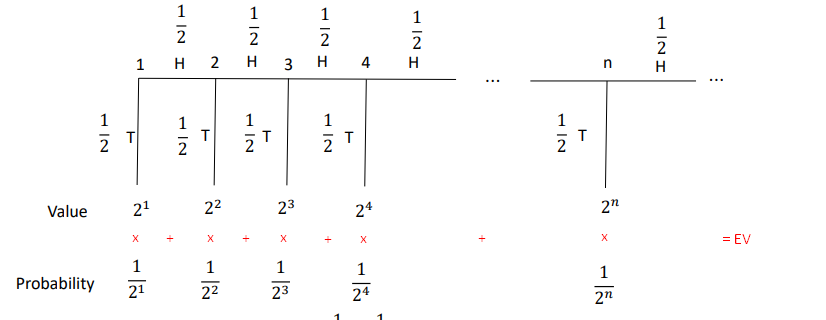
\includegraphics[width=8cm, height=6cm]{pic27}
  \end{center}
  This is problematic since, in this case, the expected value criterion contradicts normal behaviour wherein you can make option A worth any finite amount of money and option B will still be chosen
  \par
  \underline{Change in Welfare}: the expected value criterion suggests that the change in welfare (utility) is $\partial u = \partial w$, where $w$ denotes wealth and $u$ denoted utility. By integration, this leads to the utility function $u(w) = w$
\vspace{6mm}
\subsubsection{Expected Utility Criterion}
The expected utility criterion (from Bernoulli) can be used to evaluate lotteries, where the expected utility of a lottery $p$ with possible outcomes in $Z$ is defined as
\begin{gather*}
  EU(p) = \sum_{z \in Z} p_{z}u(z)
\end{gather*}
where $p_{z}$ is the probability of the outcome $z$ and $u(\cdot) = \ln (\cdot)$. This has the welfare of a lottery increasing based on what percentage it increases your wealth
\par \vspace{0.3em}
  \underline{Change in Welfare}: the change in welfare $\partial u$ is equal to the percentage change in wealth, that is $\partial u = \tfrac{\partial w}{w}$. By integration, this leads to the utility function $u(w) = \ln (w)$
  \par
  \underline{St Petersburg Resolution}: using the expected utility criterion, option A is valued at $EU(A) = \ln(1000)$ and option B is valued at $EU(B) = \ln (4)$ as shown below:
  \begin{align*}
    EU(B) &= \frac{1}{2} \ln(2) + \frac{1}{2^{2}} \ln (2^{2}) + \dots + \frac{1}{2^{n}} \ln (2^{n}) \\
    &= \frac{1}{2} \ln(2) + \frac{2}{2^{2}} \ln(2) + \dots + \frac{n}{2^{n}} \ln (2)
    &= (\frac{1}{2} + \frac{2}{2^{2}} + \dots + \frac{n}{2^{n}}) \ln(2) \\
    &= 2 \ln(2)
  \end{align*}
  Therefore, the expected utility criterion suggests we should choose option A as $\ln (1000) > \ln(4)$. This solves the St Petersburg Paradox
  \par
\vspace{6mm}
\subsubsection{Expected Utility Theory}
Suppose that $Z = \left\{ z_{1}, \dots, z_{n} \right\}$ is finite. In this case, a lottery can be described as a point $p = (p_{1}, \dots, p_{n}) \in \mathbb{R}_{+}^{n}$ with the restriction that
\begin{gather*}
  \sum_{i=1}^{n}p_{i} = 1
\end{gather*}
to give us a probability distribution over all elements in Z
\par \vspace{0.3em}
  \underline{Set of Lotteries}: now the set of lotteries is $L = \left\{ p = (p_{1}, \dots, p_{n}) \in \mathbb{R}_{+}^{n}: \sum_{i=1}^{n} p_{i}=1 \right\}$ and is denoted by $\Delta (Z)$
  \par
  \underline{Set Properties}: the set of lotteries is a compact convex subset of $\mathbb{R}_{+}^{n}$
  \begin{itemize}
    \item \underline{Logic}: this is as $0 \leq p \leq 1$ for all $p$'s in the set (i.e. is bounded), the set contains all the end points as the sum of all $p$'s must be 1 (i.e. is closed), and the average of any two points in the set is contained in the set (i.e. is convex where any $p$ can be represented as the sum of smaller $p$'s and it contains all possible incomes since an income not attainable just has $p=0$)
    \item  \underline{Proof}: for $Z = \left\{ z_{1}, \dots, z_{n} \right\}$ as a finite set of prizes, we want to prove that the set of lotteries $\Delta (Z) = \left\{ p \in \mathbb{R}_{+}^{n}: \ \sum_{i=1}^{n} p_{i} = 1 \right\}$ is a convex subset of $\mathbb{R}_{+}^{n}$. Let $p,q \in \Delta (Z)$ and $\alpha \in [0,1]$, we want to show that $\alpha p + (1- \alpha)q \in \Delta(Z)$. \\
    To do this, it suffices to show that $\alpha p_{i} + (1-\alpha) q_{i} \geq 0$ for all $i = 1, \dots, n$ and $\sum_{i=1}^{n} [\alpha p_{i} + (1-\alpha)q_{i}] = 1$ - whereby we would have that $\left\{ \alpha p + (1-\alpha)q \in \mathbb{R}_{n}^{+}: \sum_{i=1}^{n}[\alpha p_{i} + (1- \alpha)q_{i} ] = 1 \right\}$ which matches the definition of $\Delta(Z)$. \\
    Since $\alpha \in [0,1]$, $p, q \in \Delta(Z)$, and $p_{i},q_{i} \geq 0$ for $i = 1, \dots, n$ then it follows that $\alpha p_{i} + (1-\alpha) q_{i} \geq 0$ for all $i = 1, \dots, n$ \\
    Since $\alpha \in [0,1]$, $p, q \in \Delta(Z)$, $\sum_{i=1}^{n} p_{i} = 1$, and $\sum_{i=1}^{n}q_{i} = 1$ then it follows that
    \begin{gather*}
      \sum_{i=1}^{n} [\alpha p_{i} + (1-\alpha)q_{i}] = \alpha (\sum_{i=1}^{n} p_{i}) + (1-\alpha)(\sum_{i=1}^{n} q_{i}) = \alpha (1) + (1- \alpha)(1) = 1
    \end{gather*}
    Given this, it must be that the set of lotteriest is a convex subset of $\mathbb{R}_{+}^{n}$
  \end{itemize}
  \par
\vspace{6mm}
\subsubsection{Expected Utility Maximizer (EUMs)}
We assume that individuals evaluate lotteries by comparing the expected utility of those lotteries. Therefore, we define an individual with preferences $\succeq$ over the set of lotteries $L$ to be an expected utility maximizer if and only if there exists a utility function $u: Z \rightarrow \mathbb{R}$ such that for all lotteries $p,q \in L$:
\begin{gather*}
  p \succeq q \Leftrightarrow \sum_{i=1}^{n} p_{i}u(z_{i}) \geq \sum_{i=1}^{n} q_{i}u(z_{i})
\end{gather*}
where the utility function $u: Z \rightarrow \mathbb{R}$ represents the preferences $\succeq$ over $L$ if the probabilities are given (i.e. objective)
\par \vspace{0.3em}
  \underline{Objective vs Subjective Uncertainty}: in the objective case we can compare lotteries using only $u$ since the utility function will holistically indicate how the individual compares lotteries with the probability distribution being given. In the subjective case we have that the probabilities are uncertain themselves, dependent on the individuals beliefs, and so we cannot rely solely on the utility function $u$ to represent preferences $\succeq$
  \par
  \underline{Wealth and Lottery Decisions}: the outcome $z_{i}$ must take into account the total wealth of the individual under the lottery. That is, if the lottery was being purchased using the individuals wealth $w$ then we would include the cost of the lottery $x$ in the calculation of $u(z_{i})$
  \par
  \underline{Expected Utility Representation}: for an expected utility maximizer with preferences $\succeq$ over the set of lotteries $L$, there is a function $v: L \rightarrow \mathbb{R}$ such that for all $p,q \in L$ we have
  \begin{gather*}
    v(p) \geq v(q) \Leftrightarrow  p \succeq q
  \end{gather*}
  where $v(p) = \sum_{i=1}^{n} p_{i}u(z_{i})$ and $v(q) = \sum_{i=1}^{n} q_{i}u(z_{i})$
  \begin{itemize}
    \item  \underline{$u$ and $v$ Relationship}: let an expected utility maximizer have preferences $\succeq$ over a set of lotteries and let $u$ and $v$ be two utility functions over the set of certain outcomes that represent those preferences. Then, $u = \alpha v + \beta$ for some $\alpha \in \mathbb{R}_{+}$ and $\beta \in \mathbb{R}$
    \item  \underline{Preferences Implication}: the function $v(\cdot)$ is continuous which suggests from our preferences over bundles results that the preferences are complete, transitive, and continuious
    \item  \underline{Linear Sum Implication}: the utility function over lotteries is required to be a linear sum of the certain utilities
  \end{itemize}
  \par
  \underline{Existence of a Lottery Utility Representation}: by assuming complete, transitive, and continuious preferences on the lottery space $L$ we get a utility representation over those lotteries
  \begin{itemize}
    \item  \underline{Logic}: from our preferences over bundles results we know that if preferences are complete, transitive, and continuous on a closed convex subset $X$ pf $\mathbb{R}_{+}^{n}$, then there is a utility representation of those preferences. Since the set of lotteries $L$ is a subset of $\mathbb{R}_{+}^{n}$, the expected utility maximizer problem is similar to that of preferences over bundles we can infer the above
    \item  \underline{Note}: we require the independence axiom for this to be in the form of expected utility
  \end{itemize}
  \par
  \underline{Expected Utility Theorem (Confirming EUMs)}: a person with preferences $\succeq$ over $L$ is an expected utility maximizer (i.e. their utility representation takes the above form) if and only if the preferences satisfy axioms A1, A2, and A3
  \begin{itemize}
    \item  \underline{Axiom 1}: $\succeq$ are complete and transitive
    \item  \underline{Axiom 2}: $\succeq$ are continuious in the sense that for all $p \in L$; the at least as good as set $G(p) = \left\{ q \in L: q \succeq p \right\}$ and the weakly worse than set $W(p) = \left\{ q \in L: p \succeq \right\}$ are closed in $L$
    \item  \underline{Axiom 3}: we have independence where for all $p, q, r \in L$ and all $\alpha \in (0,1)$ we have that:
    \begin{gather*}
        p \succeq q \Leftrightarrow \alpha p + (1 - \alpha)r \succeq \alpha q (1 - \alpha)r
    \end{gather*}
    \begin{itemize}
      \item  \underline{Translation}: $p \succeq q$ implies that any compound lottery located between $p$ and some arbitrary element $r$ is weakly preferred to any compound lottery located between $q$ and the same arbitrary element $r$. Note that $\alpha$ determines the location of the compound lotteries and the same relationship should be true in the other direction
      \item  \underline{Logic}: the preferences between two lotteries should not be affected by some identical part in the two lotteries
    \end{itemize}
  \end{itemize}
  \par
  \underline{Example of Axiom Violation}: suppose we have $p, q, r$ where $q$ is the status quo, $p$ is the status quo plus $100$, and $r$ is the total destruction of the universe. Therefore we have that $p \succ q \succ r$ and by the intermediate value theorem $\exists \alpha \in (0,1)$ such that $\alpha p + (1- \alpha)r \sim q$. This is not feasible since no one is likely to take a gamble on the total destruction of the universe and so the indifference $\sim$ would not hold. Since the intermediate value theorem does not hold, we have that either continuity or completeness is violated
\vspace{6mm}
\subsubsection{Lottery Illustration}
Consider the finite set of outcomes $Z = \left\{ (1,1), (1,2), (3,0) \right\}$ where we take $z_{1} = (1,1)$, $z_{2} = (1,2)$, and $z_{3} = (3,0)$. Suppose we use the Cobb-Douglas utility function $u(x_{1}, x_{2}) = x_{1}x_{2}$ such that we have a certain outcome (i.e. $z_{1} = (1,1)$ has the utility $u(1,1) = 1$) \par \vspace{6mm}
  \underline{Lottery Probability Representation}: a lottery over these 3 bundles can be represented by a triple $p = (p_{1}, p_{2}, p_{3}) \in \Delta (Z)$
  \begin{itemize}
    \item  \underline{Example}:suppose that the triple $p = (\tfrac{1}{2}, \tfrac{1}{3}, \tfrac{1}{6})$ is a lottery that puts probability $\tfrac{1}{6}$ on bundle $(3,0)$, $\tfrac{1}{3}$ on bundle $(1,2)$, and $\frac{1}{2}$ on bundle $(1,1)$. Using Cobb-Douglas, the expected utility of $p = (\tfrac{1}{2}, \tfrac{1}{3}, \tfrac{1}{6})$ is $EU(p) = \tfrac{1}{2}(1) + \tfrac{1}{3}(2) + \tfrac{1}{6}(0) = \tfrac{7}{6}$
  \end{itemize}
  \par
  \underline{Certain Outcomes Reduction}: to preserve the same lottery space ($\mathbb{R}^{+}_{n}$), we can extend the space of $p$ when considering a certain outcome
  \begin{itemize}
    \item  \underline{Example}: the certain outcome $(1,1)$ can be represented by the triple $(1,0,0)$ which puts probability 1 on the bundle $(1,1)$
  \end{itemize}
  \par
  \underline{Compound Lotteries Reduction}: to preserve the same lottery space ($\mathbb{R}^{+}_{n}$), we can take the convex combination within a compound lottery
  \begin{itemize}
    \item  \underline{Example}: if we put probability $\tfrac{1}{2}$ on the lottery $(\tfrac{1}{2}, \tfrac{1}{3}, \tfrac{1}{6})$ and $\tfrac{1}{2}$ on the lottery $(1,0,0)$ to form a new lottery then we have a lottery over a lottery (i.e. a compound lottery). If we take the convex combination of our compound lottery we have:
    \begin{gather*}
      \bigg((\frac{1}{2})\frac{1}{2} + (\frac{1}{2})1, (\frac{1}{2})\frac{1}{3} + (\frac{1}{2})0, (\frac{1}{2})\frac{1}{6} + (\frac{1}{2})0 \bigg) = (\frac{3}{4}, \frac{1}{6}, \frac{1}{12})
    \end{gather*}
  \end{itemize}
  \par
\vspace{6mm}
\subsubsection{Risk Attitudes and Lotteries over Money}
If the set $Z \subseteq \mathbb{R}$ (i.e. is a lottery over money), then the shape of the utility function $u: Z \rightarrow \mathbb{R}$ reveals the following risk attitudes of an individual: \\
\null\quad \textit{Strictly Risk Adverse} iff the person prefers the expected value of a lottery to the lottery itself \\
\null\quad \textit{Risk Neutral} iff the person is indiffferent between the expected value of a lottery and the lottery itself \\
\null\quad \textit{Strictly Risk Loving} iff the person prefers the lottery itself to the expected value of the lottery \par \vspace{0.3em}
  \underline{Shape of U-function Implication}: an expected utility maximizer is strictly risk adverse/loving/neutral if and only if his utility function over certain outcomes is strictly concave/convex/linear
\vspace{6mm}
\subsubsection{Exercise 1}
Consider a decision maker who is an expected utility maximizer with a utility function over wealth $w > 0$ defined as $u(w) = \ln w$ \par \vspace{0.3em}
  \begin{itemize}
    \item  \underline{Question 1}: is the decision maker risk neutral, strictly risk averse, or strictly risk loving
    \begin{itemize}
      \item  \underline{Answer}: the decision maker is risk adverse since $u(w) = \ln w$ is strictly concave over values $w > 0$. Note that if we instead had $w \geq 0$, then $u(w) = \ln w$ would not be strictly concave and therefore for the outcome $w=0$ the decision maker would be indifferent
    \end{itemize}
  \end{itemize}
  \begin{itemize}
    \item  \underline{Question 2}: suppose the decision maker has a wealth of $w = 100$. He is considering buying a risky asset that will pay off $A = 100$ with probability $p = 0.5$ and will pay $B = 50$ with probability $(1 - p)$. Calculate the maximum amount $x$ he will be willing to pay for the risky asset
    \begin{itemize}
      \item  \underline{Answer}: we have from the lottery that:
      \begin{align*}
        EU(p) &= \sum_{z} p_{z} u(z) \\
        &= p \ln (A + 100 - x) + (1 - p) \ln (B + 100 - x) \\
        &= 0.5 \ln (200 - x) + 0.5 \ln (150 -x)
      \end{align*}
      where we include $100 - x$ in the lotteries outcome to incorporate the change in wealth from the point that the lottery is engaged in, with $A - x$ or $B - X$ being the net return. If not engaging in the lottery we have that:
      \begin{gather*}
        EU(w) = \ln (100)
      \end{gather*}
      From the expected utility maximizer theory, the maximum amount that the decision maker would be willing to pay for the lottery $p$ occurs when:
      \begin{gather*}
        w \sim p \Leftrightarrow EU(w) = EU(p)
      \end{gather*}
      Therefore, the maximum amount is:
      \begin{align*}
        EU(w) &= EU(p) \\
        \ln (100) &= 0.5 \ln (200 - x) + 0.5 \ln (150 - x) \\
        9.2103 &= \ln (200 - x) + \ln (150 - x) \\
        9.2103 &= \ln ((200 - x) (150 - x)) \\
        e^{9.2103} &= 30000 - 350x + x^{2} \\
        0 &= x^{2} - 350x + 20000.4037
      \end{align*}
      Using the quadratic formula we have from the above equation that $x = 71.9224$
    \end{itemize}
  \end{itemize}
  \begin{itemize}
    \item  \underline{Question 3}: suppose now that he owns the risky asset so his wealth is either 200 or 150 depending on the outcome of the lottery he owns. What is the maximum amount $x_{s}$ he will accept for selling the asset
    \begin{itemize}
      \item  \underline{Answer}: we can derive the minimum amount that the decision maker would be willing to sell the lottery for by finding when the EU of the lottery equals the EU of the sale price of the lottery combined with wealth:
      \begin{gather*}
          s \sim p \Leftrightarrow EU(s) = EU(p)
      \end{gather*}
      Therefore the minimum amount is:
      \begin{align*}
        EU(s) &= EV(p) \\
        \ln (x + 100) &= 0.5 \ln (200) + 0.5 \ln (150) \\
        \ln (x + 100)^{2} &= \ln (200) + \ln (150) \\
        (x + 100)^{2} &= 200 \cdot 150 \\
        x &= \sqrt{200 \cdot 150} - 100 \\
        x &= 73.2055
      \end{align*}
    \end{itemize}
  \end{itemize}
  \begin{itemize}
    \item  \underline{Question 4}: consider a consumer with a utility function defined over wealth given by $u(w) = -e^{-\alpha w}$ where $\alpha > 0$. Redo the comparison between the maximum buy ($x_{b}$) and maximum sell ($x_{s}$) price with a general wealth level $w > 0$ and general payments $A$ and $B$ and general $p \in [0, 1]$. Can you make any determination about the relative sizes of $x_{s}$ and $x_{b}$ in this case?
    \begin{itemize}
      \item  \underline{Answer}: in this case for indifference between buying the asset and just having the wwealth $w$ is determined by $x^{b}$ where:
      \begin{gather*}
        u(w) = pu(w + A - x_{b}) + (1-p)u(w + B - x_{b})
      \end{gather*}
      For the utility function $u(w) = -e^{-\alpha w}$, this implies:
      \begin{gather*}
        e^{-\alpha w} = pe^{-\alpha (w + A - x_{b})} + (1-p)e^{-\alpha(w + B - x_{b})}
      \end{gather*}
      We can devide each side by $e^{-\alpha x_{b}}$ to find that $x_{b}$ solves:
      \begin{gather*}
        e^{-\alpha x_{b}} = pe^{-\alpha A} + (1-p)e^{-\alpha B} \ \tag{*}
      \end{gather*}
      For the situation where the asset is sold for a price $x_{s}$ we have the following indifference condition:
      \begin{gather*}
        u(w + x_{s}) = pu(w + A) + (1-p)u(w + B)
      \end{gather*}
      For the utility function $u(w) = -e^{-\alpha w}$, this implies:
      \begin{gather*}
        e^{-\alpha (w + x_{s})} = p e^{-\alpha (w + A)} + (1-p)e^{- \alpha (w + B)}
      \end{gather*}
      We can devide each side by $e^{-\alpha}$ to find that $x_{s}$ solves:
      \begin{gather*}
        e^{-\alpha x_{s}} = pe^{-\alpha A} + (1-p)e^{-\alpha B} \ \tag{**}
      \end{gather*}
      Equating the RHS of equations ($*$) and ($**$) we conclude that $x_{s} = x_{b}$. Incidentally, this utility function exhibits constant relative risk aversion (like linear utility functions, i.e. risk neutral ones). For any utility function in this class the buying and selling prices are the same and independent of the initial wealth. However, note that for general utility functions this is not the case.
    \end{itemize}
  \end{itemize}
\par
\vspace{6mm}
\subsubsection{Exercise 2}
The independence axiom states that for all lotteries $p,q,r $ and all $\alpha \in (0,1)$:
\begin{gather*}
  p \succeq q \Leftrightarrow \alpha p + (1-\alpha)r \succeq \alpha q + (1-\alpha)r
\end{gather*}
Show that this axiom implies that for all lotteries $p,q,r$ and $\alpha \in (0,1)$:
\begin{gather*}
  p \succ q \Leftrightarrow \alpha p + (1-\alpha)r \succ \alpha q + (1-\alpha)r
\end{gather*}
\par \vspace{0.3em}
  \begin{itemize}
    \item  \underline{Proof of $p \succ q \Rightarrow$}: using the contrapositive method of proof we want to show that if $\alpha p + (1 - \alpha) r \nsucc \alpha q + (1- \alpha)r$ then $p \nsucc q$. \\
    If $\alpha p + (1 - \alpha) r \nsucc \alpha q + (1- \alpha)r$ it follows that either:
    \begin{align*}
      (1):& \ \ \alpha p (1-\alpha)r \lnot \succeq \alpha q + (1-\alpha) r \\
      (2):& \ \ \alpha p (1-\alpha)r \succeq \alpha q + (1-\alpha) r
    \end{align*}
    If (1) holds then, by the contrapositive of the ($\Rightarrow$) independence axiom, $p \lnot \succeq q$. Therefore, by the definition of $\succ$, $q \succ p$ which means that $p \nsucc q$. \\
    If (2) holds then, by ($\Leftarrow$) independence axiom, $q \succeq p$. Therefore, by the definition of $\succeq$, $p \nsucc q$ since either $q \sim p$ or $q \succ p$. \\
    Overall, the results of the two possible cases cases demonstrate that
    \begin{gather*}
      \alpha p + (1 - \alpha) r \nsucc \alpha q + (1- \alpha)r  \Rightarrow p \nsucc q
    \end{gather*}
    which being a contrapositive means that:
    \begin{gather*}
      p \succ q \Rightarrow \alpha p + (1-\alpha)r \succ \alpha q + (1-\alpha)r
    \end{gather*}
    \item  \underline{Proof of $\alpha p + (1-\alpha)r \succ \alpha q + (1-\alpha)r \Rightarrow$}: using proof by contradition, suppose that:
    \begin{gather*}
      \alpha p + (1-\alpha)r \succ \alpha q + (1-\alpha)r \Rightarrow p \nsucc q
    \end{gather*}
    Since $\alpha p + (1-\alpha)r \succ \alpha q + (1-\alpha)r$ it follows that by the definition of $\succeq$ that $\alpha p + (1-\alpha)r \succeq \alpha q + (1-\alpha)r$. By the ($\Leftarrow$) independence axiom this implies that $p \succeq q$ which, combined with the fact $\begingroup\color{magenta} p \nsucc q \endgroup$, implies that $q \succeq p$. \\
    Since $q \succeq p$ it follows from the ($\Rightarrow$) independence axiom that $\alpha q + (1-\alpha)r \succeq \alpha p + (1-\alpha)r \Rightarrow$. This contradicts the statements that $p \nsucc q$ occurs when $\alpha p + (1-\alpha)r \succ \alpha q + (1-\alpha)r \Rightarrow$ and therefore it must be that:
    \begin{gather*}
      \alpha p + (1-\alpha)r \succ \alpha q + (1-\alpha)r \Rightarrow p \succ q
    \end{gather*}
    \begingroup\color{magenta} doesn't $p \nsucc q$ necessitate that $q \succeq p$ on its own without the prior statement \endgroup
  \end{itemize}
\par
\vspace{6mm}
\subsubsection{Exercise 3}
Prove that if a decision maker is an expected utility maximizer, then the independence axiom is satisfied \par \vspace{0.3em}
\begin{itemize}
  \item  \underline{Approach/Guide}: since the decision maker is an expected utility maximizer, her preferences $\succeq$ over the set of lotteries $L$ satisfy that for all $p,q \in L$
  \begin{gather*}
    p \succeq q \Leftrightarrow \sum_{i=1}^{n} p_{i}u(z_{i}) \geq \sum_{i=1}^{n} q_{i}u(z_{i})
  \end{gather*}
  for some real valued utility function $u$ over the set of certain alternatives $Z$. We need to show that these preferences satisfy the independence axiom where for all $p,q,r \in L$ and all $\alpha \in (0,1)$: $p \succeq q \Leftrightarrow \alpha p + (1-\alpha)r \succeq \alpha q + (1-\alpha)r$
  \item  \underline{Answer}: let $p,q,r \in L$ and $\alpha \in (0,1)$. By the decision maker being an expected utility maximizer, we have that:
  \begin{gather*}
    p \succeq q \Leftrightarrow \sum_{i=1}^{n} p_{i}u(z_{i}) \geq \sum_{i=1}^{n} q_{i}u(z_{i}) \ \tag{1}
  \end{gather*}
  By simple calculation we have the following result:
  \begin{gather*}
    \sum_{i=1}^{n} p_{i}u(z_{i}) \geq \sum_{i=1}^{n} q_{i}u(z_{i}) \Leftrightarrow \sum_{i=1}^{n} (\alpha p_{i} + (1- \alpha) r_{i})u(z_{i}) \geq \sum_{i=1}^{n} (\alpha q_{i} + (1- \alpha) r_{i})u(z_{i}) \ \tag{2}
  \end{gather*}
  Given equations $(1)$ and $(2)$, we can conclude that:
  \begin{gather*}
    p \succeq q \Leftrightarrow \alpha p + (1-\alpha)r \succeq \alpha q + (1-\alpha)r
  \end{gather*}
\end{itemize}



\newpage

\section{Producer Theory}







\end{document}
